\documentclass{article}
%% packages
\usepackage{arxiv}
\usepackage[utf8]{inputenc} % allow utf-8 input
\usepackage[T1]{fontenc}    % use 8-bit T1 fonts
\usepackage{hyperref}  
% hyperlinks
\usepackage{url}            % simple URL typesetting
\usepackage{booktabs}       % professional-quality tables
\usepackage{amsfonts}       % blackboard math symbols
\usepackage{nicefrac}       % compact symbols for 1/2, etc.
\usepackage{microtype}      % microtypography
% \usepackage{subcaption}
\usepackage{balance}  % to better equalize the last page
\usepackage{graphicx} % for EPS, load graphicx instead
% \usepackage{times}    % comment if you want LaTeX's default font
\usepackage{url}      % llt: nicely formatted URLs
\usepackage{caption}
\usepackage{soul}
\usepackage{color}
\usepackage{subfig}
\usepackage{amsmath}
\usepackage{float}
\usepackage{cleveref}
\usepackage{textcomp}
\usepackage[T1]{fontenc}
\usepackage{lineno}
\usepackage[dvipsnames]{xcolor}
\usepackage[authoryear,round]{natbib}
% \usepackage{apacite}
%%
%% end of the preamble, start of the body of the document source.
\begin{document}

% \title{Just-in-time: gaze guidance behavior while action planning and execution in VR}
\title{Task Complexity Affects Gaze Guidance Behavior while Action Planning and Execution in Naturalistic VR}
\author{
  Ashima Keshava\\
  University of Osnabr{\"u}ck\\
  Germany\\
  \texttt{akeshava@uos.de} \\
  %% examples of more authors
   \And
   Farbod Nosrat Nezami\\
  University of Osnabr{\"u}ck\\
  Germany
  
  %% examples of more authors
   \And
   Henri Neumann\\
  SALT AND PEPPER \\ Software GmbH \& Co.KG.\\
  Germany\\
  %% examples of more authors
   \And
  Krzysztof Izdebski\\
  SALT AND PEPPER \\ Software GmbH \& Co.KG.\\
  Germany\\
   \And
   Thomas Sch{\"u}ler\\
  SALT AND PEPPER \\ Software GmbH \& Co.KG.\\
  Germany\\
  %% examples of more authors
   \And
   Peter K{\"o}nig\\
   University of Osnabr{\"u}ck\\
   University Medical Center,\\ Hamburg-Eppendorf\\
   Germany
}

\maketitle

\begin{abstract}
Eye movements in the natural environment have primarily been studied for over-learned everyday activities such as tea-making, sandwich making, driving that have a fixed sequence of actions associated with them. These studies indicate an interplay of low-level action schemas that facilitate task completion. However, it is unclear if this strategy is also in play when the task is novel and a sequence of actions must be planned in the moment. To study attention mechanisms in a novel task in a natural environment, we recorded gaze and body movement data in a virtual environment while subjects performed a sorting task where they sorted objects on a life-size shelf based on some object features. To study the action planning and execution related gaze guidance behavior we also controlled the complexity of the sorting task by introducing EASY and HARD tasks. We show that subjects are close to optimal while performing EASY trials and are more sub-optimal while performing HARD tasks. Fixations aligned with action onset show task complexity elicits greater proportion of look-ahead, and monitoring fixations but not directing and guiding fixations. Task complexity affected the scan-paths on the task-relevant regions of interest during action planning and execution where subjects exhibit a greater search and action monitoring behaviors in HARD tasks and less so in EASY tasks. Task complexity also affected the temporal sequence of first fixations on the task-relevant regions of interest systematically for action planning but not for action execution. Our findings show that task complexity modulates the competition of low-level cognitive schemas during planning and execution even when sub-optimal decisions are made by the actor.
\end{abstract}

\keywords{action planning, gaze-guided planning, gaze control, action schemas, virtual reality}

% \linenumbers
\captionsetup[figure]{font=scriptsize,labelfont=bf}
\section{Introduction}

Humans actively use vision during everyday activities to gather and refine information about the environment.Since the seminal works of \citet{Yarbus2013-eu} and \citet{Buswell1935-di} there has been consistent evidence that eye movements depend on the viewing task the observer is performing. This is further supplemented by studies that have revealed that overt attention during natural viewing conditions is driven by scene semantics i.e. meaning and not by salience \citet{Henderson2017-it}. \citet{Kollmorgen2010-wg} have also shown that spatial viewing biases and task dependent features contribute highly to attention in a visual scene. We have growing evidence that eye movements are driven by top-down factors of task relevance and less by bottom-up factors of salience in the environment.

While studying eye movements profiles on static images in a controlled lab environment has offered illuminating insights into task-relevant modulation of attention, mobile subjects can give us a richer picture of cognitive processing in more naturalistic settings. In a pragmatic turn in cognitive science, there is a greater push towards incorporating the study of cognitive processes while interacting with the external world \citet{Parada2020-ys}. Moreover, \citet{Engel2013-bx} proposed that cognition encompasses the body and in turn, bodily action can be used to infer cognition. To this effect, understanding the control of eye movements in natural, real-life situations requires a mobile setup that allows for a subject to be recorded in tandem with volitional actions in a controlled yet unconstrained environment. In recent years, virtual reality (VR) and mobile sensing has offered great opportunity to create controlled, natural environments where subjects' eye and body movements can be measured reliably along with their interactions with the environment \citep{Keshava2020-cp, Clay2019-cu, Mann2019-ls}. Experiments in virtual environments have grown popular in recent years and have shown promise towards studying cognition in naturalistic and controlled environments.

Seminal studies have already investigated eye movement behavior in natural environment with fully mobile participants. For example, eye movements have been studied under a plethora of natural condition while walking \citep{Matthis2018-ho}, tea-making \citep{Land1999-ol} , sandwich making \citep{Hayhoe2003-lw} , driving \citep{Mars2012-bn, Sullivan2012-gg}, hand-washing \citep{Pelz2001-cn} , hitting a ball \citep{Land2000-pw}. For these studies head-mounted eye-tracking devices were used as participants performed these tasks that allowed for fully mobile interaction with the world. Although the head mounted camera and eye-tracker record the subjects' ego-centric view of the environment, there are still some deficiencies in precisely recording the changes in the environment simultaneously with bodily interactions in a unified space. Here, VR based studies can provide a unique solution to monitor time-resolved changes in the environment and the participant.

Experiments in naturalistic settings have revealed several distinct functions of the eye movements during everyday tasks. In the pioneering studies of \citet{Land1999-ol} and \citet{Hayhoe2003-lw}, subjects performed everyday activities of tea-making and sandwich-making, respectively. These studies required a sequence of actions which involved manipulating objects one at a time to achieve the goal. Both studies showed that nearly all the fixations were task-related. Furthermore, there was a systematic relative timing of visual fixation on object and manipulation where fixations were made to target objects about 600ms before manipulation. More importantly, \citet{Ballard1995-ji} proposed a \emph{"just-in-time"} strategy that universally applies to this relative timing of fixations and actions. In other words, they state that fixations that provide information for a particular action immediately precede that action and is crucial for a fast and economical execution of the task.

\citet{Land2001-do} posit that fixations can be broadly categorized into four functional groups; 'locating' fixations which retrieve visual information; 'directing' fixations which acquire the position information of an object and accompany a manipulation action and facilitate reaching movements; 'guiding' fixations which alternate between two objects being manipulated e.g. knife, bread, and butter; and 'checking' fixations which monitor where the task-constraints in the scene have been met. These findings have also been corroborated by \citet{Pelz2001-cn, Mennie2007-my} .

\citet{Pelz2001-cn} showed similar just-in-time strategy of gaze allocation while performing a hand-washing task. They also reported a small number of fixations ~5\% that did not serve the immediate sub-task but rather provided information that would be needed for a future action. The authors hypothesize these "look-ahead" fixations provide a mechanism to stabilize the visual input stream that result from a sequence of actions, facilitate task-switching, and reduce conscious effort required to complete the actions in a sequence. Hence, look-ahead fixations can be explained as a perceptual strategy to ease the cognitive load attending to complex tasks in the real world. In sum, the wide-ranging functions of eye movements are well documented in natural and routine tasks.

\citet{Land2001-do} have also proposed a framework that outlines that flow of visual and motor control during task execution as shown in Figure \ref{fig:land_schema}. The process summarizes the various operations that \emph{must} occur during an 'object-related action' i.e., individual actions performed on separate objects to achieve the desired goal. As described in Land (2006) each schema " specifies the object to be dealt with, the action to be performed on it, and the monitoring required to establish that the action has been satisfactorily completed." Further, the gaze control samples the information about the location and identity of the object and directs the hands to it. Subsequently, the motor control system of the arms and hands implement the desired actions. Here, vision provides the information of where to direct the body, which state to monitor, and determine when the action must be terminated. Taken together, a 'script' of instructions is sequentially implemented where the eye movements earmark the task-relevant locations in the environment that demand attentional resources for at action.

\begin{figure}[h]
    \centering
    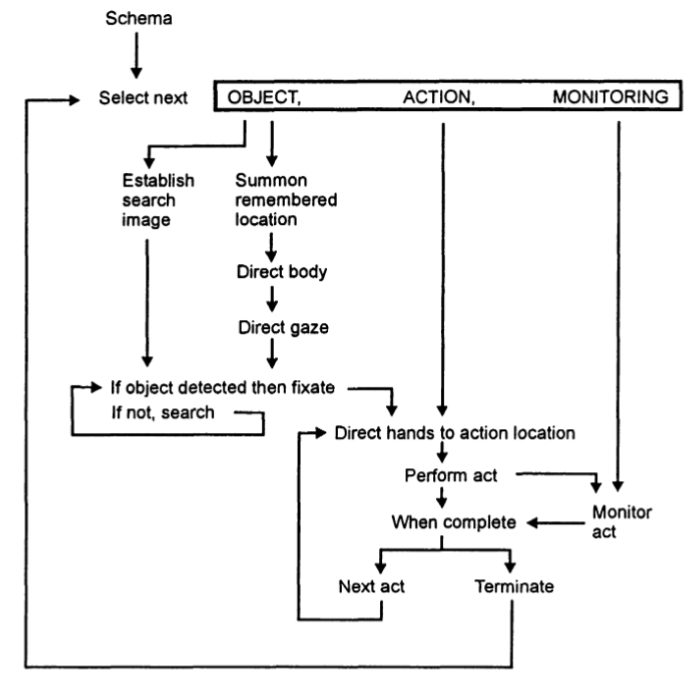
\includegraphics[width=0.6\linewidth]{source/figures/introduction/land_schema.PNG}
    \caption{Schematic of motor and gaze control systems during performance of natural tasks. From \citet{Land2001-do}}
    \label{fig:land_schema}
\end{figure}

The common theme in the above studies is that the tasks (tea-making, sandwich-making, hand-washing) have an organized task structure. These tasks involve specific object-related actions such as picking up the knife, picking up the teapot, etc. and have a predefined 'script' for the execution of the tasks. The studies, therefore, study eye movements that are under strict control of a task sequence. Moreover, these tasks are over-learned and over-generalized as they are part of a habitual action repertoire for an adult human being. As discussed by \citet{Land2006-da} these low level schemas defined above are likely not executed under deliberate conscious control. This distinction corresponds to \citet{james2007principles}'s distinction between "ideo-motor" and "willed" acts. As James described, ideo-motor actions correspond to movements where we are "aware of nothing between the conception and execution" of the said action. In contrast, the willed actions require "an additional conscious element in the shape of a fiat, mandate, or expressed consent." Hence, it is unclear whether these low-level schemas of gaze control operate similarly for deliberate actions where an internal task 'script' is not already known.

\citet{Norman1986-qb} proposed a theoretical framework for the components of attentional mechanisms that govern deliberate/planned actions. In comparison to the low-level schema proposed by Land \& Hayhoe which can account for routine, well-learned tasks, the \citet{Norman1986-qb} model suggests another supervisory module that selects a schema to implement. In well-learned tasks, a schema is triggered automatically without conscious control. However, when a task is fairly complex and requires planning, multiple low-level schemas might compete for resources at the same time and require \emph{contention scheduling}. For example, contentions can arise on whether to monitor the current action with respect to previous actions or future planned actions to fulfill the task-relevant goals. Such a scheduling mechanism is then required to provide conflict resolution for potentially relevant schemas either by inhibition or activation. Additionally, the model proposes a Supervisory Attentional System (SAS) that modulates the selection of a schema. The model suggests that attentional resources are deployed only at the specific points in a task where schema selection is required. Taken together, the model predicts that a failure of the supervisory control can lead to an instability of attention and heightened distraction.

In the present study, we investigate the mechanisms of allocation of attention while performing a novel task in a naturalistic environment. We created two types of tasks that varied in complexity and required performing a sequence of actions to accomplish the cued goal. We asked subjects to sort objects on a life-size shelf based on the object features. The complexity of the task depended on sorting based on one object feature or both. We designed the tasks to be novel in a way that subjects had to plan their action sequences on-the-fly and in absence of a pre-defined action "script". We concurrently measured the eye and body movements while subjects performed the tasks. 

Based on the models proposed by \citet{Land2001-do} and \citet{Norman1986-qb}, we predicted four behavioral outcomes:
\begin{enumerate}
    \item if the actions are deliberately and optimally planned, subjects would exhibit targeted gaze guidance towards task-relevant objects. Conversely, eye movement would be more random when actions are produced randomly and without deliberation.
    \item optimal planning of action would require gaze allocation to target locations of previous actions to monitor task requirements are validated by current actions.
    \item with optimal selection of relevant action schemas, subjects would allocate gaze to task-locations relevant to the actions in the future action sequence.
    \item given optimal gaze allocation towards current task-relevant locations would not be just-in-time i.e. fixations on the target objects would immediately precede an action. 
\end{enumerate}

Overall, these predictions generalize the flow of low-level schemas proposed by \citet{Land2001-do} by taking into account a novel task which forces deliberate action planning.




\section{Methods}
\subsection{Participants}
A total of 60 participants (39 females, mean age = 23.9 ± 4.6 years) were recruited from the University of Osnabr{\"u}ck and the University of Applied Sciences Osnabr{\"u}ck. Participants had a normal or corrected-to-normal vision and no history of neurological or psychological impairments. They either received a monetary reward of €7.50 or one participation credit per hour. Before each experimental session, subjects gave their informed consent in writing. They also filled out a questionnaire regarding their medical history to ascertain they did not suffer from any disorder/impairments which could affect them in the virtual environment. Once we obtained their informed consent, we briefed them on the experimental setup and task. The Ethics Committee of the University of Osnabr{\"u}ck approved the study. 

\subsection{Apparatus \& Procedure}
For the experiment, we used an HTC Vive Pro Eye head-mounted display (HMD)(110° field of view, 90Hz, resolution 1080 x 1200 px per eye) with a built-in Tobii eye-tracker\footnote{\href{https://enterprise.vive.com/us/product/vive-pro-eye/}{https://enterprise.vive.com/us/product/vive-pro-eye-office/}}. Participants used an HTC Vive controller to manipulate the objects during the experiment with their right hand. The HTC Vive Lighthouse tracking system provided positional and rotational tracking and was calibrated for 4m x 4m space. For calibration of the gaze parameters, we used 5-point calibration function provided by the SRanipal SDK. To make sure the calibration error was less than $1^\circ$, we performed a 5-point validation after each calibration. Due to the study design, which allowed a lot of natural body movements, the eye tracker was calibrated repeatedly during the experiment after every 3 trials. Furthermore, subjects were fitted with HTC Vive trackers on both ankles, both elbows and, one on the midriff. The body trackers were also calibrated subsequently to give a reliable pose estimation using inverse kinematics of the subject in the virtual environment. We designed the experiment using the \hl{Unity3D\footnote{\href{www.unity.com}{Unity, www.unity.com}}  2018.x.x (version)} and SteamVR game engine and and controlled the eye-tracking data recording using HTC VIVE Eye Tracking SDK SRanipal\footnote{\href{https://developer.vive.com/resources/vive-sense/sdk/vive-eye-tracking-sdk-sranipal/}{SRanipal, developer.vive.com/resources/vive-sense/sdk/vive-eye-tracking-sdk-sranipal/}} (v1.1.0.1)
\begin{figure}[H]
    \centering
    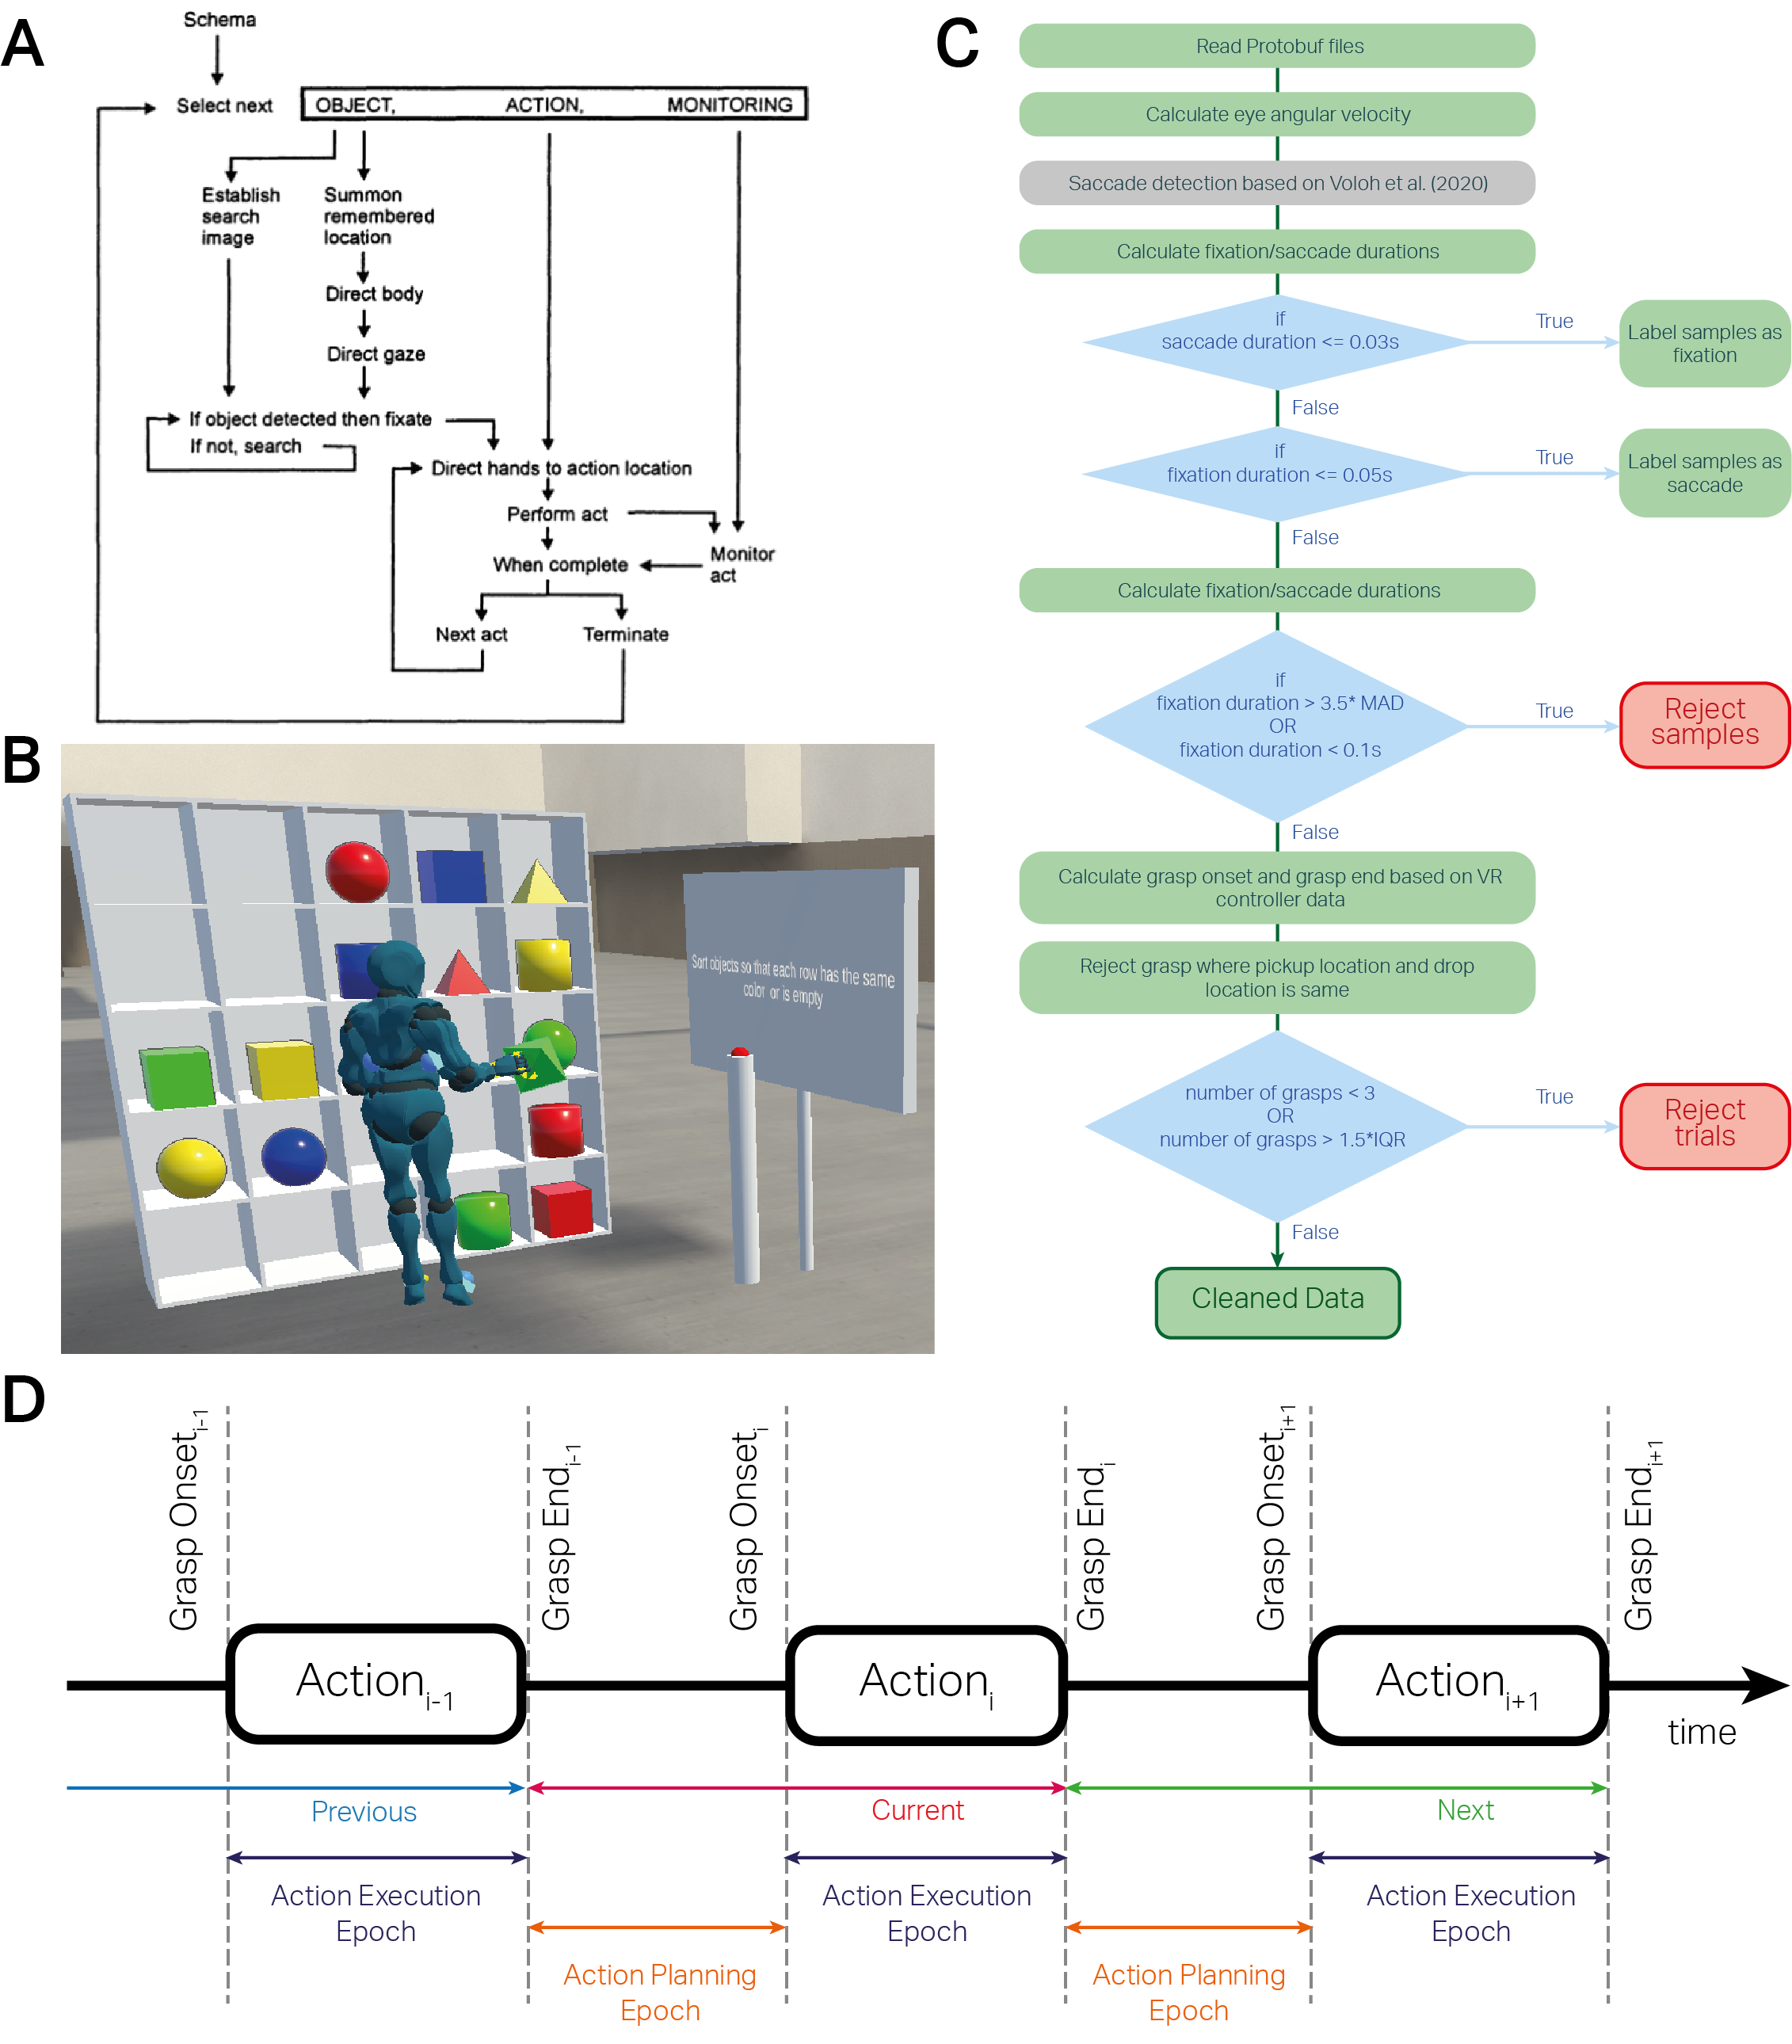
\includegraphics[width=1\linewidth]{source/figures/experiment_setup/Methods_1.png} \\
    \caption[]{\textbf{A.} Schematic of motor and gaze control during performance of natural tasks \citet{Land2001-do}. \textbf{B.} Experimental Task. In a virtual environment participants sorted 16 different objects based on 2 features color or shape while we measured their eye and body movements. The objects were randomly presented on a 5x5 shelf at the beginning of each trial and were cued to sort objects by shape and/or color. Trials where objects were sorted based on just one object feature (color or shape) were categorized as EASY trials. Conversely, in the trials where sorting was based on both features (color and shape) were categorized as HARD trials. All participants performed 24 trials in total (16 easy trials and 8 hard trials) with no time limit. \textbf{C.} Data preprocessing steps for fixation/saccade detection and data rejection. \textbf{D.} Action execution and planning epochs. In order to study the function of eye movements we divided each trial into action planning and action execution epochs. The action execution epochs start from grasp onset till grasp end for each object displacement, whereas the action planning epochs start from grasp end of previous object displacement and grasp onset of current object displacement.}
    \label{figure:task}
\end{figure}



The experimental setup consisted of 16 different objects placed on a shelf of 5x5 grid. The objects were differentiated based on two features: color and shape. We used four high contrast colors (red, blue, green and yellow) and four 3D shapes (cube, sphere, pyramid and cylinder). The objects had an average height of 20cm and width of 20cm. The shelf was designed with a height and width of 2m with 5 rows and columns of equal height, width and, depth. Participants were presented with a display board on the right side of the shelf where the trial instructions were displayed. Subjects were also presented with a red buzzer that they could use to end the trial once they finished the task. 



\subsection{Experimental Task}
Subjects performed two practice trials where they familiarized themselves with handling the VR controller and the general aspects of the setup. In these practice trials they were free to explore the virtual environment and handle the objects. After the practice trials, subjects were asked to sort object based on the one and/or two features of the object. There were two types of trials: EASY and HARD. Subjects were not limited by time to complete the task. Each subject performed 24 trials with each trial type (as listed below) randomly presented twice throughout the experiment. 
The EASY trials instructions were as follows:
\begin{enumerate}
    \item Sort objects so that each row has the same shape or is empty
    \item Sort objects so that each row has all unique shapes or is empty
    \item Sort objects so that each row has the same color or is empty
    \item Sort objects so that each row has all unique colors or is empty
    \item Sort objects so that each column has the same shape or is empty
    \item Sort objects so that each column has all unique shapes or is empty
    \item Sort objects so that each column has the same color or is empty
    \item Sort objects so that each column has all unique colors or is empty
\end{enumerate}
The HARD trials instructions were as follows:
\begin{enumerate}
    \item Sort objects so that each row has all the unique colors and all the unique shapes once
    \item Sort objects so that each column has all the unique colors and all the unique  shapes once
    \item Sort objects so that each row and column has each of the four colors once. 
    \item Sort objects so that each row and column has each of the four shapes once. 
\end{enumerate}


\subsection{Data pre-processing}

\subsubsection{Gaze Data}

The data preprocessing steps are illustrated in \ref{fig:task}C. As a first step, using eye-in-head 3d gaze direction vector for the cyclopean eye we calculated the gaze angles for the horizontal $\theta\textsubscript{h}$ and vertical $\theta\textsubscript{v}$ directions. All of the gaze data was sorted by the timestamps of the collected gaze samples. The 3d gaze direction vector of each sample is represented in $(x, y, z)$ coordinates as a unit vector that defines the direction of the gaze in VR world space coordinates. In our setup, the x coordinate corresponds to the left-right direction, y in the up-down direction, z in the forward-backward direction. The formulas used for computing the gaze angles are as follows:

 \begin{equation}\label{eq:h_angle}
     \theta\textsubscript{h} = \frac{180}{\pi} * \arctan{\frac{x}{z}}
 \end{equation}   
  \begin{equation}\label{eq:v_angle}
     \theta\textsubscript{v} = \frac{180}{\pi} * \arctan{\frac{y}{z}} 
 \end{equation}   
 
Next, we calculated the angular velocity of the eye in both the horizontal and vertical coordinates by taking a first difference of the angular velocity and dividing by the difference between the timestamp of the samples using the formula below:
\begin{equation}\label{eq:h_vel_angle}
    \omega\textsubscript{h} = \Delta\theta\textsubscript{h} / \Delta t
 \end{equation}  
 \begin{equation}\label{eq:v_vel_angle}
     \omega\textsubscript{v} = \Delta\theta\textsubscript{v} / \Delta t
 \end{equation}  

Finally, we calculated the magnitude of the angular velocity ($\omega$) at every timestamp from the horizontal and vertical components using:
\begin{equation}\label{eq:vel_angle}
     \omega = \sqrt{\omega_h^2 + \omega_v^2}
 \end{equation}  

To filter the samples where gaze was relatively stable, we used an adaptive threshold method for saccade detection described by \citet{Voloh2019-oc}. We selected an initial saccade velocity threshold $\theta\textsubscript{0}$ of 200 $\circ$/sec. All eye movement samples with an angular velocity of less than $\theta\textsubscript{0}$ were used to compute a new threshold $\theta\textsubscript{1}$. $\theta\textsubscript{1}$ was three times the median absolute deviation of the selected samples. If the difference between $\theta\textsubscript{1}$ and $\theta\textsubscript{0}$ was less than 1 $\circ$/sec $\theta\textsubscript{1}$ was selected as the saccade threshold else, $\theta\textsubscript{1}$ was used as the new saccade threshold and the above process was repeated. This was done until the difference between $\theta\textsubscript{n}$ and $\theta\textsubscript{n+1}$ was less than or equal to 1 $\circ$/sec. This way we arrived at the cluster of samples that belonged to fixations and the rest were classified as saccades. After this, we calculated the duration of the fixations and saccades. To handle miniscule fixations and saccades, we labeled all samples with saccade duration less than 0.03 seconds as a fixation. We also labeled all fixation samples with duration of less than 0.05 seconds as saccades. Following this, we recalculated the fixation and saccade durations. Finally, we rejected all fixations with duration greater than 3.5 times the median absolute deviation of the population fixation duration as well as fixations that were less than 0.1 seconds long. 


\subsubsection{Grasp data}

Subjects used the trigger button of the HTC vive controller to virtually grasp the objects on the shelf and displace them to other locations. In the data, the trigger was recorded as a boolean which was set to TRUE when a grasp was initiated and was reset to FALSE when the grasp ended. Using the position of the controller in the world space, we determined the locations from the shelf where a grasp was initiated and ended. We also removed trials where the controller data was showed implausible locations in the world space. These faulty data can be attributed to loss of tracking during the experiment. Next, we removed grasping periods where the beginning and final locations of the objects on the shelf were the same. We calculated the inter-quartile range (IQR) of the participants object displacement behavior for the two trial types (EASY and HARD). To remove the outlying object displacements in the trials, we removed the trials with 1.5 times the IQR of object displacements. We also removed those trials with fewer than three object displacements. 

\subsection{Data Analysis}\label{sec:data_analysis}

In order to study the function of eye movements for both action planning and execution, we divided each trial into 2 types of epochs. The action execution epoch spanned the time from start of object displacement to the end. The action planning epochs started from end of previous object displacement to start of current object displacement. The schematic of this epoch creation is illustrated in figure \ref{figure:task}D. This division of time within each trial into separate epochs allows us to parse the role of overt eye movements in planning and execution of object related actions separately.

For the action planning and execution epochs, we examined the spatial and temporal characteristics of eye movements while performing the sorting tasks. We divided the object and shelf locations into 7 regions-of-interest (ROIs) comprising of previous, current, and next target object and target shelf. More specifically, the previous target object refers to the object that was handled in the previous action epoch, and previous target shelf as the shelf where the previous target object was placed. Similarly, the current target object refers to the object that is picked up and placed on the target shelf in the current epoch and the next target object and next target shelf in the immediately following epoch. All other regions which did not conform to the above 6 ROIs are categorized as 'other' and not relevant to the action sequence.  As we need at least 3 object related actions within a trial to form the ROIs for the action planning and action execution epochs, we removed trials where subjects made fewer than three object displacements. In this format, we could parse the sequence of eye movements on the seven ROIs that are relevant for planning and execution of the object related actions. 


% \subsubsection{Task-based behavioral differences}\label{sec:behavior}

% In order to assess the planning behavior of the participants, we determined the optimal object displacements required to accomplish the tasks for the two trial type. To determine the optimal object displacements we designed a depth-first search algorithm that computed the minimum number of displacements required to sort the objects for the 5000 random initial configurations of 16 objects in 25 shelf locations for both EASY and HARD trial constraints. We compared the mean number of object displacements made by the participants in the EASY and HARD trials with the model based object displacements using independent t-tests.

% Next, we tested the differences in the duration of 
\subsubsection{Action Locked Gaze Control}\label{sec:avg_fixations}

We were interested in the average fixation behavior time-locked to action initiation. For each grasp onset in a trial we chose the time period from 2 seconds before grasp onset and 2 seconds after. We divided this 4 second period into bins of 0.15 seconds and calculated the number of fixations on the seven ROIs described above. For each time bin, we calculated the proportion of fixations on the ROIs per trial type (EASY, HARD). To find the time-points where there were significant differences between EASY and HARD trials for a given ROI, we used the cluster permutation method. Here, we use the t-statistic as a test statistic for each time-bin, where t is defined as:

\begin{gather*}\label{eq:cluster_permutation}
 t = \sqrt{N} * \frac{x}{\sigma}
 \end{gather*}

and, x is the mean difference between the trial types, and $\sigma$ is the standard deviation of the mean and N is the number of subjects. We used a threshold for t at 2.14 which corresponds to the t-value at which the p-value is 0.05 in the t-distribution. We first found the time-bins where the t-value was greater than the threshold. Then, we computed the sum of the t-values for these clustered time-bins which gave a single value that represented the mass of the cluster. Next, to assess the significance of the cluster, we permuted all the time-bins across trials and subjects and computed the t-values and cluster mass for 1000 different permutations. This gave us the null distribution over which we compared the cluster mass shown by the real data. To account for the multiple independent comparisons for the seven ROIs, we considered the significant clusters to have a Bonferroni corrected p-value less than 0.007 (0.05/7). In the results, we report the range of the significant time-bins for the seven ROIs for the two trial types the corresponding p-values. 

\subsubsection{Spatio-temporal Gaze Control in Action Planning and Execution}\label{sec:transitions}

To compute the scan paths within the action planning and execution epochs we created transition matrices that show the origin and destination locations of the fixations on the 7 ROIs. We used the steps described by \citet{Hooge2013-bk} to first create the scan paths and then the transition matrices. We calculated the transition matrices summarizing gaze transitions from and to the 7 ROIs from the action planning and execution epochs for each object displacement. Using the transition matrices, we calculated the net and total transitions from and to each ROI. For every transition matrix 'A' per trial, net and total transition are defined as follows:
\begin{equation}\label{eq:net_transitions}
     A_{net} = A - A^T
\end{equation}  
\begin{equation}\label{eq:total_transitions}
     A_{total} = A + A^T
\end{equation}  

As discussed in \citet{Hooge2013-bk}, if subjects make equal number of transitions between all ROIs, we can expect no transitions in the net transition matrix and can surmise that the gaze was allocated more randomly. Conversely, with strong gaze guidance we would expect more net transitions. Hence, using the net and total transitions per trial, we then calculated the relative net transitions as:

\begin{equation}\label{eq:f_value}
     Relative_{Transitions} = \frac{\sum A_{net}}{\sum A_{total}}
\end{equation}  

We then took the mean of the relative transitions per trial as a measure of gaze guidance in that trial. Higher mean relative transitions would indicate gaze allocated to ROIs in a systematic manner whereas, relative transitions would represent a random gaze allocation towards the ROIs.

Further, we also calculated the time required to first fixation on the 7 ROIs in a given planning or execution epoch. We then took the median time to first fixation per trial that would indicate time to first fixate on the ROIs for 50\% of the action planning and action execution epochs. This method was used by \citet{Montfoort2007-oa} and further applied by \citet{Hooge2013-bk} to capture the gaze attraction power of ROIs. As the action planning and execution epochs varied in duration, we normalized the time points by dividing them by the duration of the epoch. This way, time elapsed since start of an epoch is comparable to all epochs across trials and subjects.


\subsubsection{Linear Mixed Effects Models} \label{sec:lmm}
We modelled the linear relationship of the relative net transitions dependent on trial type (EASY, HARD), epoch type (planning, execution) and number of object displacements and their interactions. All within-subject effects were modeled with random intercept and slopes grouped by subject. The categorical variables trial type and epoch type were effect coded \citep{Schad2018-av}, so that the model coefficients could be interpreted as main effects. The object displacement variable which pertained to the number of object displacements in the trial were coded as a continuous numeric variable and centered on zero mean. The model fit was performed using restricted maximum likelihood (REML) estimation \citep{Corbeil1976-qq} using the lme4 package (v1.1-26) in R 3.6.1. We used the L-BFGS-B optimizer to find the best fit using 20000 iterations. Using the Satterthwaite method \citep{Luke2017-pz}, we approximated degrees of freedom of the fixed effects. The full model in Wilkinson notation \citep{Wilkinson1973-ex}  is defined as:

\begin{gather}\label{eq:lmm_formula1}
     Relative_{Transitions} \sim 1 + trial\_type * epoch\_type * object\_displacements \\
     + (1 + trial\_type * epoch\_type * object\_displacements | Subject ) 
\end{gather} 


We modelled the linear relationship of the median time to first fixation dependent on trial type (EASY, HARD) and the 7 ROIs and their interactions. We computed two models for the action planning and execution epochs as the. All within-subject effects were modeled with random intercept and slopes grouped by subject. The categorical variables trial\_type and ROI were effect coded, so that the model coefficients could be interpreted as main effects. For both models, we chose the latency of the first fixation on current target object as the reference factor so that the latency of the first fixation of all other ROIs could be compared to it. The model fit was performed using restricted maximum likelihood (REML) estimation \citep{Corbeil1976-qq} using the lme4 package (v1.1-26) in R 3.6.1. We used the L-BFGS-B optimizer to find the best fit using 20000 iterations. Using the Satterthwaite method \citep{Luke2017-pz}, we approximated degrees of freedom of the fixed effects. The full model in Wilkinson notation \citep{Wilkinson1973-ex}  is defined as:

\begin{gather}\label{eq:lmm_formula2}
     Fixation_{time} \sim 1 + trial\_type * ROI \\
     + (1 + trial\_type * ROI | Subject ) 
\end{gather} 




\section{Results}

Our experiment measured the eye and body movements as participants performed a sorting task in a virtual environment. The participants sorted objects based on the color and/or shape where we modulated the task complexity into EASY and HARD trials. We further divided the trials into planning and execution epochs where participants planned the selection of the target objects to grasp and then executing the action of displacing it to target shelves, respectively. In this section, we report the behavioral and oculomotor differences of the subjects for the two task types (EASY, HARD), and the planning and execution epochs.

\subsection{Task based Behavioral Differences}
In the present study, the primary object related action was to repeatedly pickup objects and place them at a desired locations until they were sorted according to the sorting task. To account for the behavioral differences between the task complexities, we used the measure of trial duration and the number of object displacements required to completet the tasks. \textcolor{Blue}{Figure \ref{figure:easy_hard_diff}A} shows the differences in EASY and HARD trials based on the time taken to finish the sorting task. A two-sample independent t-test showed that the trial duration for the two trial types were significantly different ($t = -10.13, p < 0.001$) where EASY trials that required the objects to be sorted based on a single feature were  shorter ($Mean = 54.12 seconds, SD = 13.33$) as compared to HARD trials ($Mean = 111.57 seconds, SD = 36.92$) where subjects had to sort taking into account both features (color and shape) of the objects. 

\textcolor{Blue}{Figure \ref{figure:easy_hard_diff}B} shows the comparisons in the object displacements made by the subjects and the optimal number of displacements as elicited by the optimal model for both EASY and HARD trials. Subjects made lower number of object displacements in the EASY trials ($ Mean = 10.2, SD = 1.99$) compared to HARD trials ($Mean = 15.52, SD = 2.59$). In the EASY trials the model required lower number of object displacements ($Mean = 9.42, SD = 1.48$) displacements, whereas, in the HARD trials, model required higher number of displacements ($Mean = 11.24, SD = 2.77$). We compared the human and model performance for the two trial types using independent t-tests. In the EASY trials, there was a significant difference between the model and human object displacements ($t=3.64, p<0.001$). In the HARD trials, there was also a significant difference between the model and human performance ($t=10,61, p<0.001$). This indicates that the participants did not plan their actions optimally and might have used other heuristics to complete the task.

\begin{figure}[ht]
    \centering
    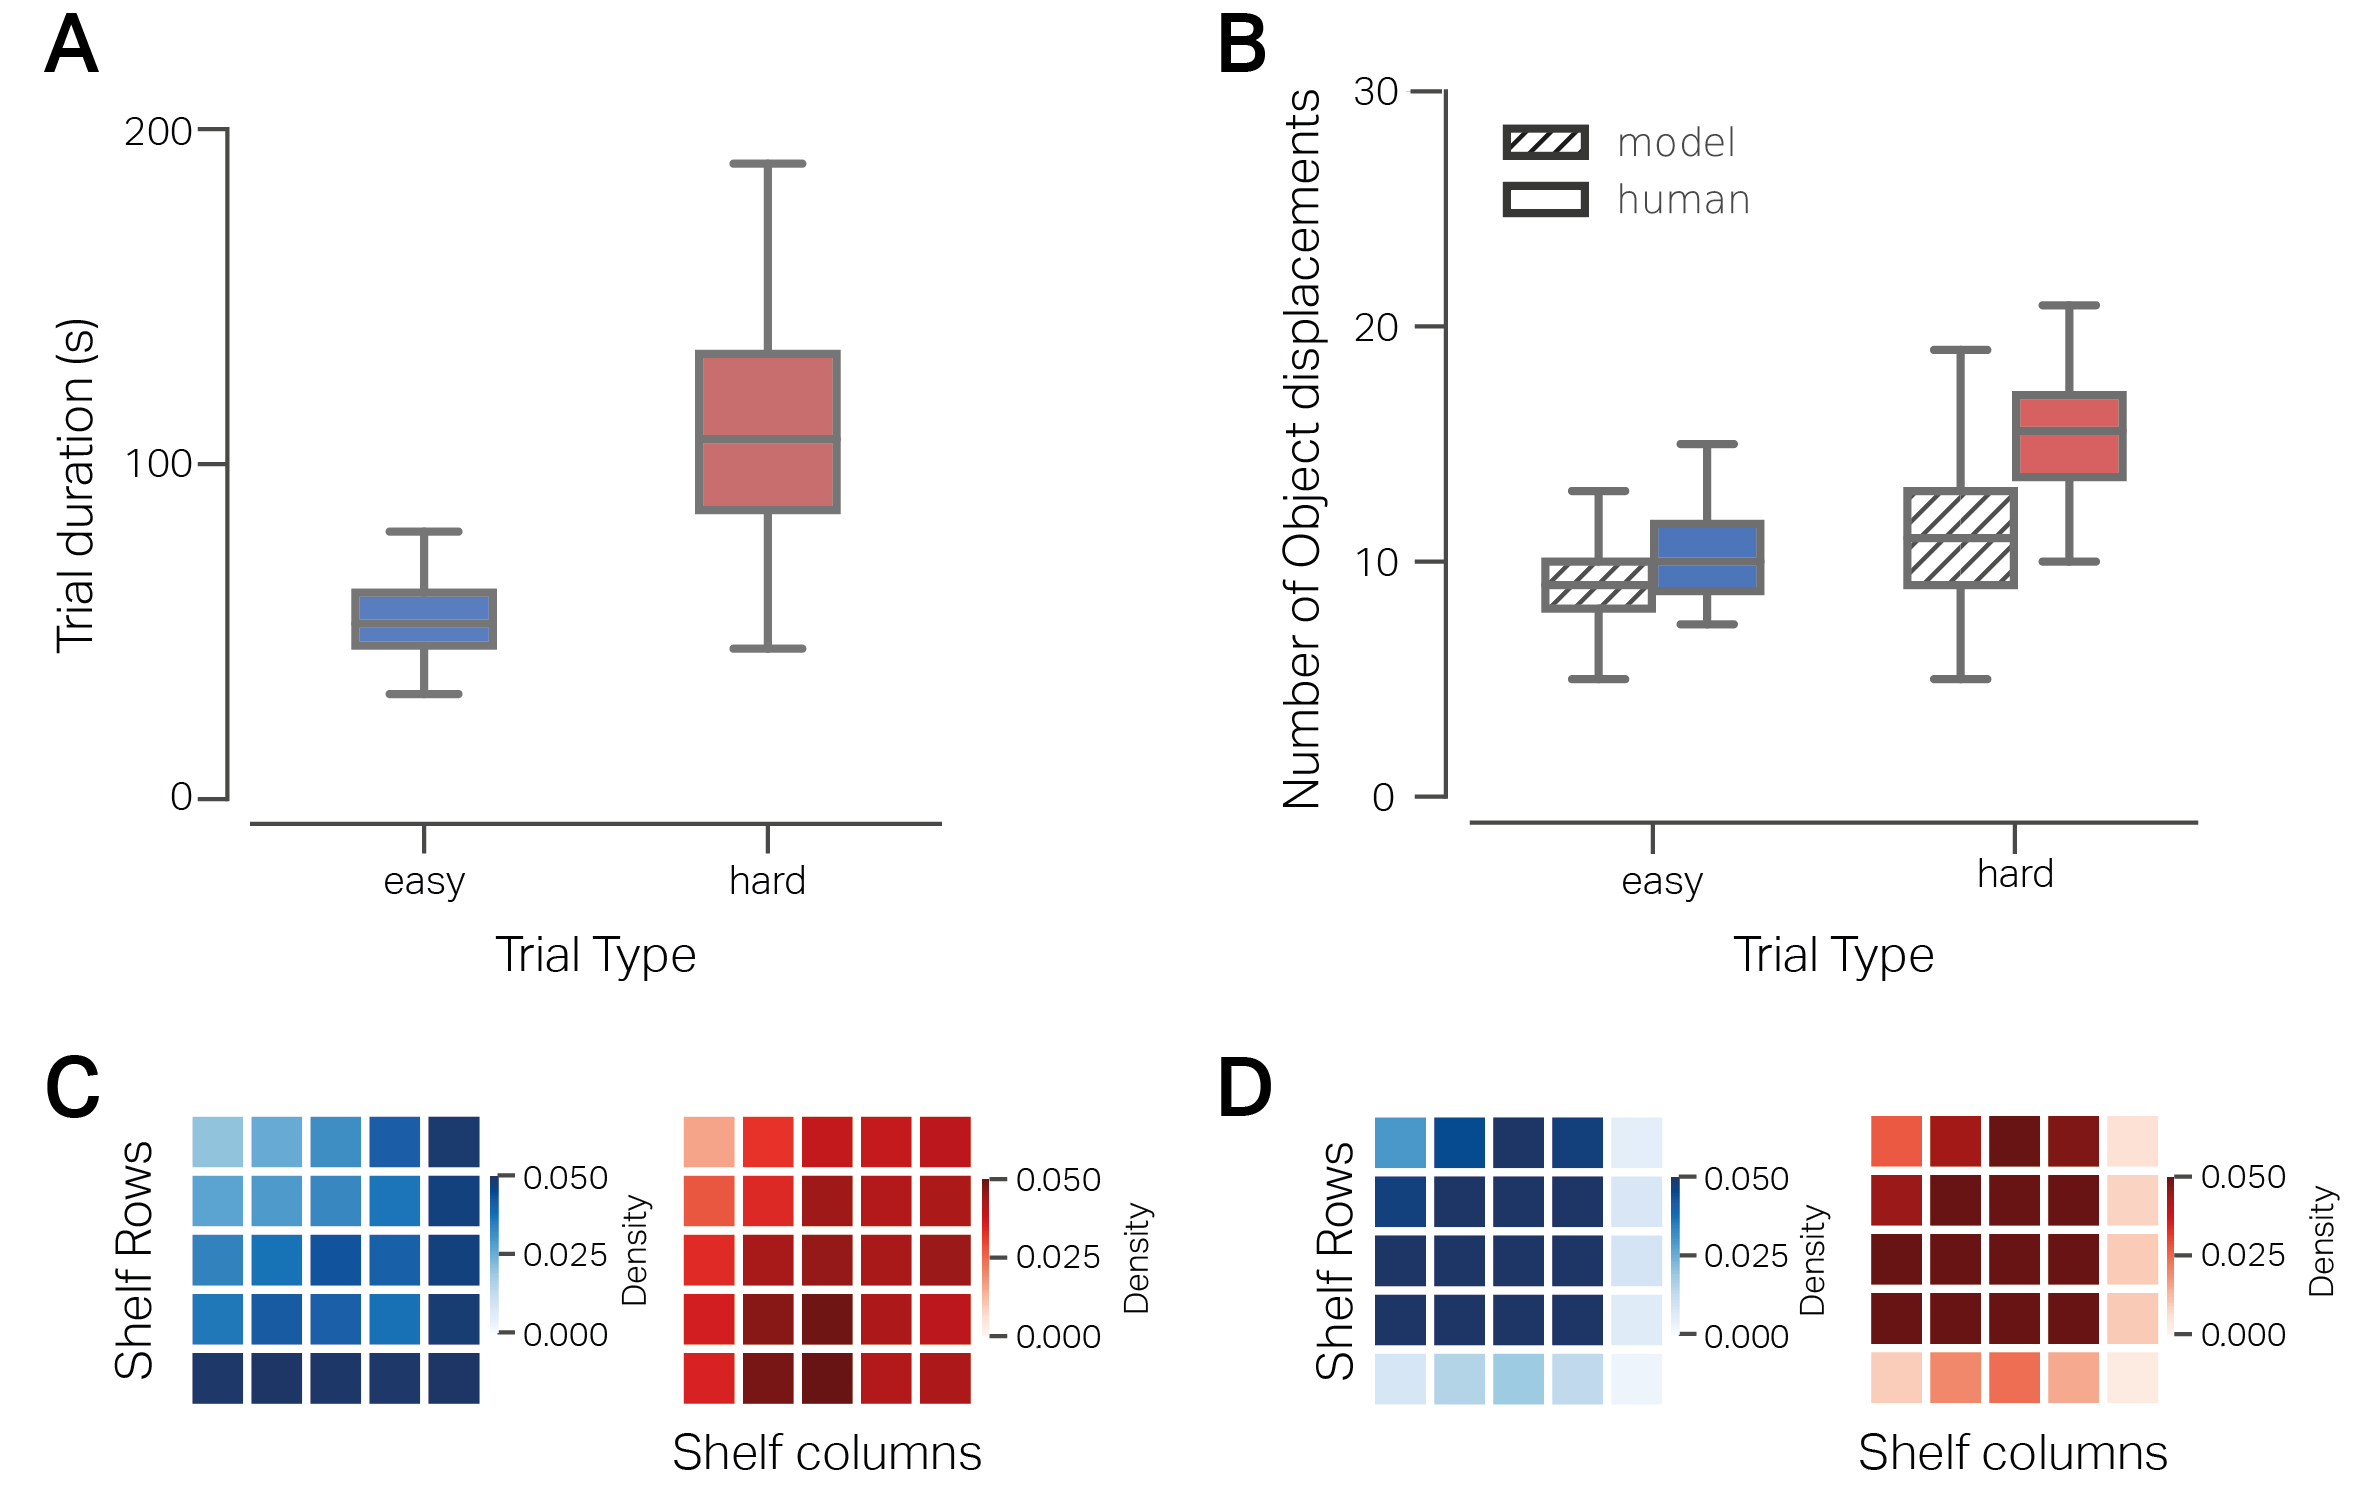
\includegraphics[width=1\linewidth]{source/figures/results/results_1.png} 
    \caption[Behavioral differences based on the 2 tasks]{\textbf{A.} Trial duration of the EASY and HARD trials. The boxplots show the inter-quartile range (IQR) of the duration of the trials for the two different trial types for all trials and participants. The whiskers represent 1.5 times the IQR. \textbf{B.} Distribution of number of object displacements for EASY (blue) and HARD (red) trials. The colored box plots show the inter-quartile range of the number of object displacements made by subjects per trial and per participant. The whiskers represent 1.5 times the IQR. The dashed box plots show optimal number of displacements required to sort the objects for a model computed with a depth-first search algorithm for 5000 random trial initialization for each trial type. \textbf{C.} Propensity of picking up objects from a preferred location on the 5x5 shelf locations with blue heatmaps showing probability density over EASY trials and red heatmaps showing density over HARD trials. The probability density shows that subjects have a propensity to pickup objects from the rightmost column and bottom column for EASY trials (left) and conversely, in the HARD trials (right) subjects pickup objects from central locations. \textbf{D.} Propensity of dropping-off objects to a preferred location on the 5x5 shelf locations with blue the heatmap showing probability density over EASY trials and red heatmap showing density over HARD trials. The probability density shows that subjects display a systematic propensity to place the objects every where other than the bottom row or rightmost column.
    }\label{figure:easy_hard_diff}
\end{figure}

To check if there were any noticeable heuristics applied by the participants, we looked into the propensity to pick-up and drop-off objects to preferred locations on the shelf. In \textcolor{Blue}{Figure \ref{figure:easy_hard_diff}C} shows that subjects preferred to pickup objects from the right-most column and bottom-most row of the shelf. \textcolor{Blue}{Figure \ref{figure:easy_hard_diff}D} shows that subjects had a propensity to drop the objects leaving out the right column and bottom row of the shelf for both EASY and HARD trials. Given the sorting tasks where subjects were presented with random initial configurations of the objects on the shelf locations, we did not expect any systematic spatial biases at play. Further, the expectation was that the subjects would move the objects randomly and not display a preference for object pickup and drop-off locations. This shows that subjects systematically, displace the objects leftward and upward employing an arbitrary heuristic to complete both task types. As the objects are instantiated on the shelf randomly, an optimal strategy would not show this behavior. We can conclude from the above that subjects offset their cognitive load of optimally completing the task by employing simple heuristics. In other words, in lieu of optimally performing the task and finishing it in a shorter time, subjects preferred to offload both cognitive  effort on the environment by adopting a more sub-optimal strategy.

% \subsection{Role of Eye Movements in Action Execution \& Planning}
\subsection{Action Locked Gaze Control}

We investigated the task complexity based differences in the the average oculomotor control over the seven ROIs time locked to the grasp onset (time when the hand makes contact with the current target object). For the analysis we chose the time period from 2s before action onset to 2s after. \textcolor{Blue}{Figure \ref{figure:action_locked}} shows the time course of proportion of fixations on the seven ROIs as described above in section \ref{sec:data_analysis} for the two trial types. The cluster permutation analysis of the time course over the ROIs for the EASY and HARD tasks revealed several time periods where the proportion of fixations were different. 

\begin{figure}[t]
    \centering
    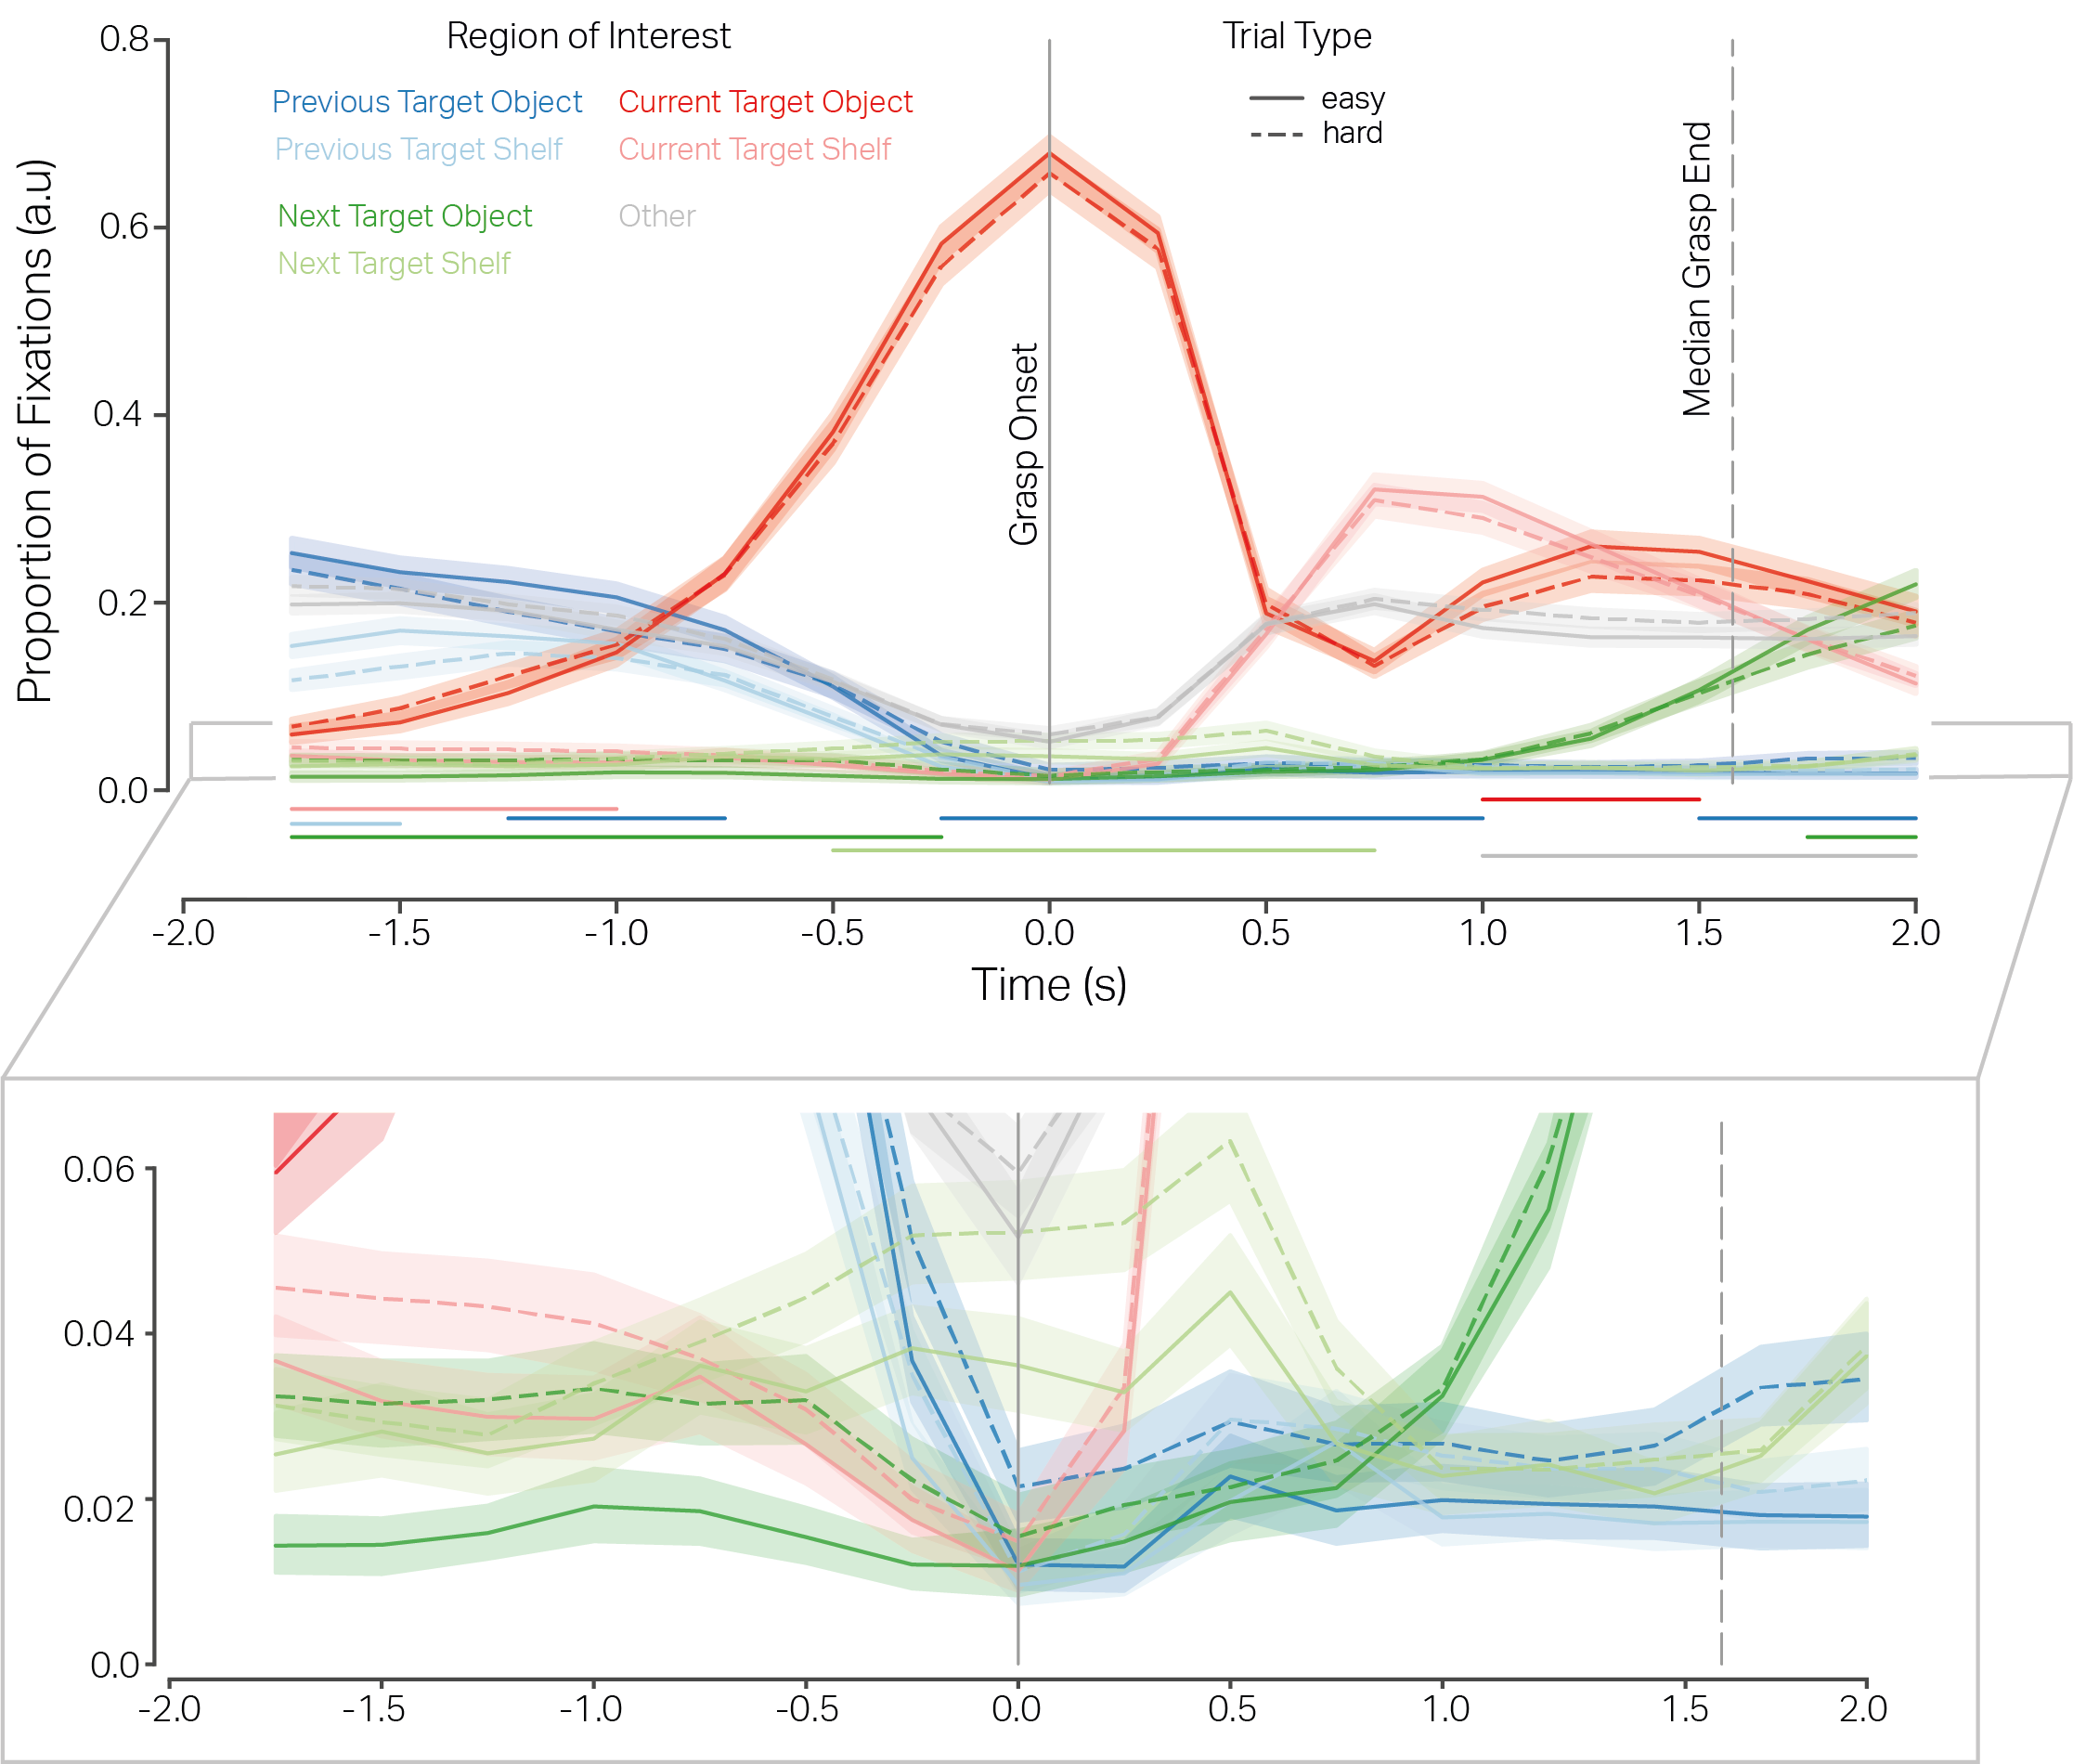
\includegraphics[width=1.\linewidth]{source/figures/results/results_23.png}
    \caption[Time course of fixations]{Proportion of fixations time-locked to the object displacement initiation (grasp onset) at time=0 and 2 seconds before and after on the seven regions of interest and for the EASY (solid trace) and HARD (dashed trace) tasks. In each time bin of 0.15s the proportion of fixations on all 7 ROIs for a trial type add up to 1. The dashed vertical line denotes the median end of the action execution phase The shaded regions show 95\% confidence interval of the mean proportion of gaze at each time-bin across all subjects. The proportion of fixations in each The horizontal traces at the bottom correspond to the significant time periods where the proportion of fixations on an ROI were different for the EASY and HARD trials.}
    \label{figure:action_locked}
\end{figure}


The proportion of fixations on the previous target object differed between EASY and HARD trials for three time periods. The first time period spanned from -1.25s to -0.75s (p-value<0.001) with lower proportion of fixations in the HARD tasks indicating allocation of gaze to other ROIs task-relevant to the action sequence. The second significant time period was from -0.25s to 1s (p-value<0.001) where the proportion of fixations were higher in the HARD tasks. This time period spans the start of the grasp onset till the execution of the object displacement strongly indicating that these fixations are related to monitoring of the execution of the current action and could be classified as 'checking' fixations. The third significant time period was from 1.5s to 2s (p-value<0.001) with higher proportion of fixations in the HARD trials. These differences might be constitutive of further 'checking' fixations in the case of HARD trials while executing the object displacement. 

The proportion of fixations on the previous target shelf were lower in the HARD trials compared to the EASY trials from -1.75s to -1.5s (p-value<0.001) before grasp onset. These differences suggest allocation of gaze to ROIs relevant to the task sequence happens earlier in the HARD tasks as more planning is required.

There were differences in the proportion of fixations on the current target object from 1s to 1.5s (p-value < 0.001) after grasp onset with lower proportion of fixations in the HARD tasks in this time period. These differences indicate that towards the end of action execution in HARD tasks fixations are allocated towards other task-relevant ROIs in the action sequence. Interestingly, there are no differences in the proportion of fixations on the current target object before the object displacement is initiated, suggesting that task complexity does not play a role in 'directing' fixations. 

There were higher proportion of fixations on the current target shelf in the HARD trials compared to EASY trials from -1.75s to -1s (p-value < 0.001) before grasp onset. These differences imply that some proportion of fixations are utilized to plan the current task, well before action has been initiated. These fixations could be classified as 'locating' fixations or look-ahead fixations which are predominantly present due to the complexity of the task. 

Similarly, there were a higher proportion of fixations on the next target object from -1.75s to -0.25s (p-value < 0.001) and a lower proportion from 1.75 s to 2s (p-value < 0.001). The differences in the first time period suggest that these fixations serve as 'locating' fixations to execute the next object displacement in the sequence. The presence of higher proportion of this fixations in the HARD tasks compared to EASY tasks indicates a need to plan the actions more thoroughly. The differences in the latter time period show a lower proportion of fixations for the HARD tasks indicating that prior locating fixations made it unnecessary to allocate attention to that object of interest. Conversely, in the EASY trials, the lower proportion of these locating fixations indicate an ad hoc gaze allocation for action execution.

There were also a higher proportion of fixations on the next target shelf from -0.5s to 0.75s (p-value < 0.001) in the HARD tasks. These fixations are made in concert with the onset of the action execution and indicate that these fixations are a play the role of both 'checking' fixations to monitor the task progression as well as 'locating' fixations to queue the locations in the scene that are important for the next action in the sequence.

Finally, the proportion of fixations on the other objects and shelves in the scene were higher in the HARD tasks from 1s to 2s (p-value < 0.001 ) after grasp onset. These differences indicate search behavior towards the end of the current task execution. Given the task complexity of the HARD trials, this search behavior might function to queue in further objects or shelves of interest in the subsequent action sequence. 


\begin{figure}[t]
    \centering
    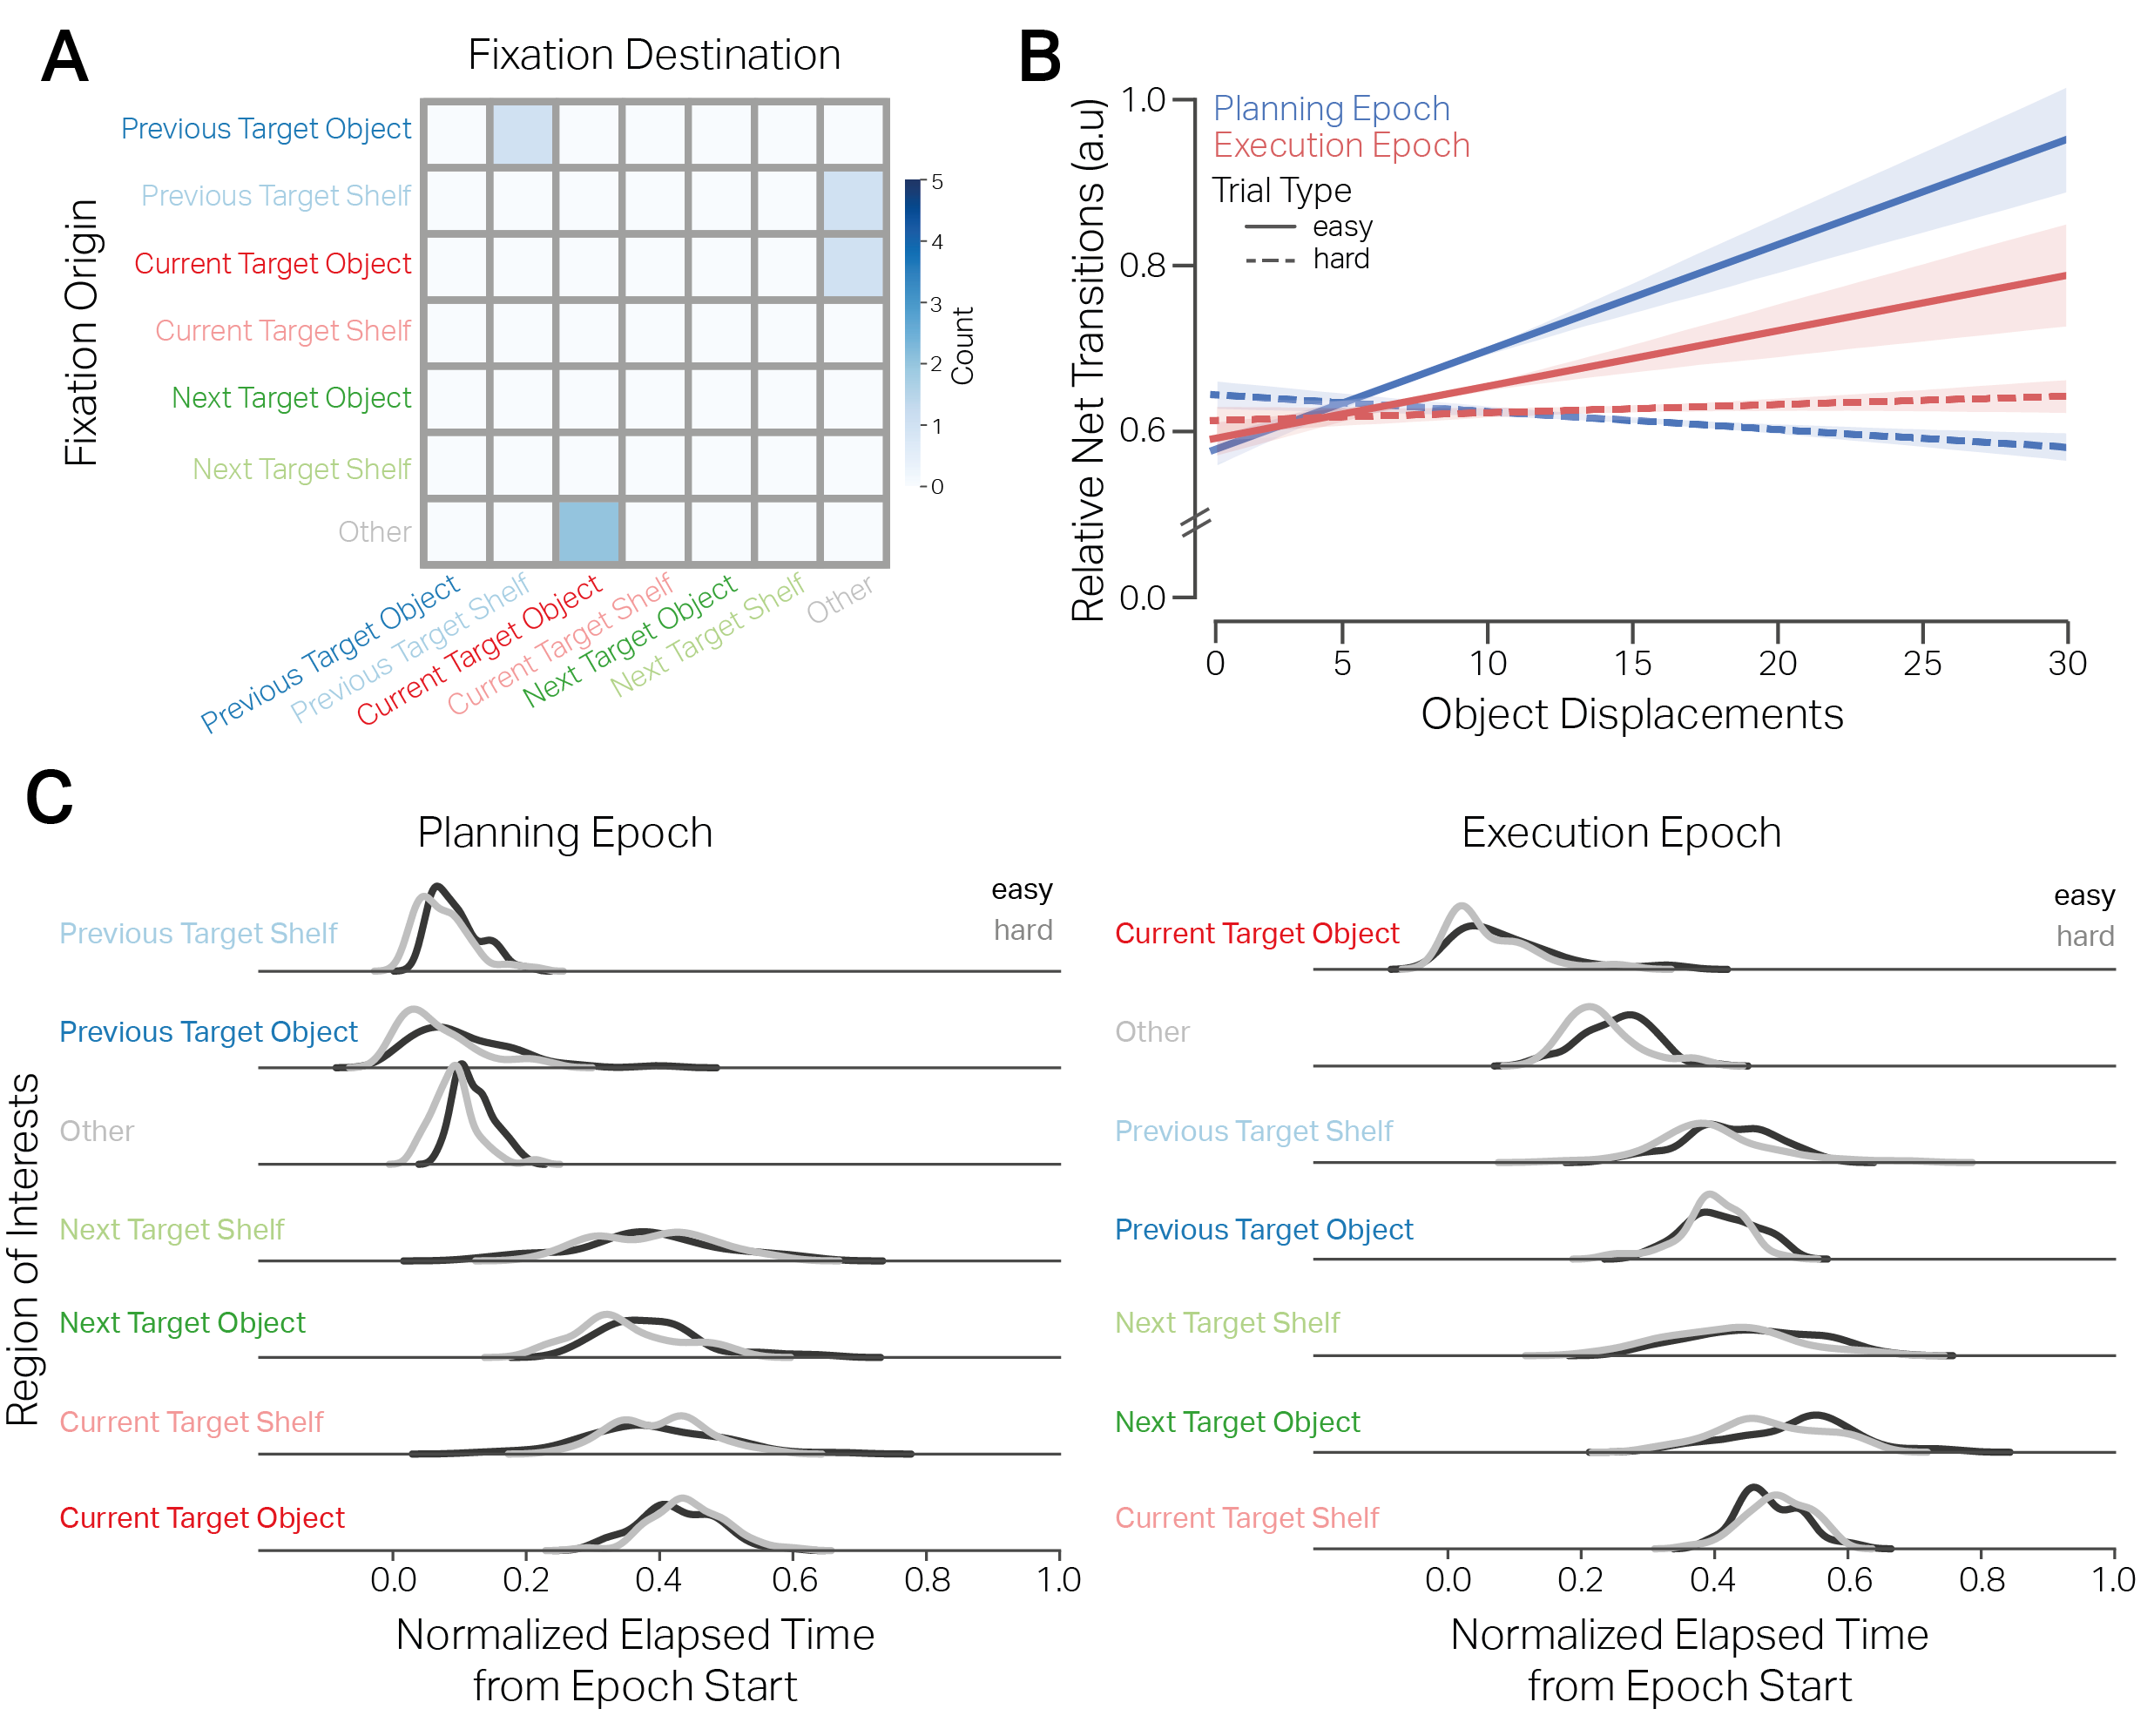
\includegraphics[width=1\linewidth]{source/figures/results/results_3.png}
    \caption[Spatiotemporal characteristics of gaze control]{\textbf{A.} Exemplar transition matrix for gaze switching in a planning epoch. The ordinate defines the origin of the gaze and the abscissa defines the destination of the gaze. \textbf{B.} Regression fit over the fixed-effects of trial types (EASY, HARD), epoch types (PLANNING, EXECUTION) and object displacements on the relative net transitions. The traces denote the the regression fit and the shaded region denotes 95\% confidence interval. \textbf{C.} Distributions of median time to first fixation on the 7 ROI for the action planning and execution epochs and trial types. The ordinate is sorted in ascending order of latency from epoch start for both planning and execution epochs. }
     \label{figure:spatiotemp}
\end{figure}


\subsection{Spatio-temporal Gaze Control in Action Planning and Execution}

The above results illustrate the average spatial and temporal aspects of attention during action planning and execution. However, the scanning behavior of subjects while they perform each action is "averaged out". In order to study the scanning behavior while subjects plan and execute an action, we computed transition matrices to capture fixations to and from each of the seven ROIs as described in Section \ref{sec:transitions}. \textcolor{Blue}{Figure \ref{figure:spatiotemp}A} shows the exemplar transition matrix for a planning epoch in an EASY trial. With the transition matrices we wanted to capture the gaze guidance behavior of the subjects while they plan and execute the actions. The relative net-transitions within the planning and execution epochs of a trial tell us the different functions of gaze guidance behaviors exhibited of the subjects. With higher relative net transitions, we expect higher gaze guidance to the current task-relevant ROIs, i.e, subjects perform saccades only for guiding their hand or body towards the current target object and less so for searching for task-relevant objects or monitoring the task. If subjects perform a search and fixate on multiple ROIs in an epoch, we would expect lower relative net transitions indicating a pattern of fixations related multiple task relevant schemas that compete for selection. 

In order to show the differences in mean gaze guidance behavior in a trial we used a linear mixed effects model (section \ref{sec:lmm}) with relative net transitions as the dependent variable and trial type (EASY, HARD), epoch type (PLANNING, EXECUTION) and number of object displacements as independent variables. As the independent variables were effect coded, the regression coefficients could be directly interpreted as main effects. \textcolor{Blue}{Figure \ref{figure:spatiotemp}B} illustrates the effects of trial type, epoch type and number of object displacements on the relative net transitions. There was a significant main effect of factor trial type (HARD - EASY) $\beta$ = -0.05 (95\%CI = [-0.06, -0.03], t(77.5)=-5.72), with a p-value < 0.001 showing that HARD trials had lower relative net transitions than EASY trials. There was also a significant main effect of factor epoch type (PLANNING - EXECUTION) $\beta$ = 0.03 (95\%CI = [0.00, 0.05], t(46.57)=-2.16), with a p-value = 0.03 showing that PLANNING epochs had higher relative net transitions than EXECUTION epochs. There was a significant effect of number of object displacements in a trial $\beta$ = 0.003 (95\%CI = [0.00, 0.01], t(57.64)=2.83), with a p-value = 0.006 showing that a one unit increase in the number of object displacements in a trial led to increase in relative net transitions by a factor of 0.003. There was a significant interaction between trial type and epoch type $\beta$ = -0.05 (95\%CI = [-0.08, -0.01], t(53.07)=-2.5), with a p-value = 0.01 showing that PLANNING epochs in HARD trials had lower relative net transitions. There was a significant interaction between trial type and number of object displacements $\beta$ = -0.009 (95\%CI = [-0.01, -0.01], t(45.82)=-4.31), with a p-value < 0.001 showing that a one unit increase in the number of object displacements in HARD trials led to increase in relative net transitions by a factor of -0.009. There was no significant interaction between epoch type and number of object displacements $\beta$ = 0.001 (95\%CI = [0.00, -0.01], t(43.20)=0.64), with a p-value = 0.52. There was a significant interaction between trial type, epoch type and number of object displacements $\beta$ = -0.01 (95\%CI = [-0.02, 0.00], t(42.67)=-2.20), with a p-value = 0.03 showing that a one unit increase in the number of object displacements in HARD trials and for PLANNING epochs led to increase in relative net transitions by a factor of -0.01.

The analysis above lends further evidence that task complexity had a significant effect on the gaze guidance behavior at the level of action planning and execution. The lower relative net transitions in the HARD tasks in general are indicative of competition between action schemas either for searching task-relevant ROIs or for monitoring the task progression. The higher relative net transitions in the EASY trials suggest saccades were primarily made towards the current task-relevant objects for directing or guiding the body or hand towards the object of interest. The significant correlation of the object displacements and the relative net transitions reveal that gaze allocation predominantly occurred in a just-in-time manner supporting the sub-optimal behavior exhibited by the subjects as well. 

To further disentangle the effect of task complexity on the order of gaze allocation to the task-relevant ROIs, we were interested in the latency of the first fixations to these . We used linear mixed effects regression to model the median time to first fixation on the 7 ROIs in each trial as described in section \ref{sec:lmm}. We modeled the latency of the first fixations for the planning and execution epochs separately. \textcolor{Blue}{Figure \ref{figure:spatiotemp}C} shows the distribution of the normalized time to first fixations on the seven ROIs for the action planning and execution epochs. 

In the action planning epoch, the time to first fixation on the previous target object was significantly earlier than the first fixation on the current target object $\beta$ = -0.35 (95\%CI = [-0.37, -0.32], t(49.67)=-29.01), with a p-value < 0.001. Similarly, the time to first fixation on the previous target shelf was significantly earlier than the first fixation on the current target object $\beta$ = -0.35 (95\%CI = [-0.37, -0.33], t(65.96)=-37.82), with a p-value < 0.001. The time to first fixation on other ROI was significantly earlier than the first fixation on the current target object $\beta$ = -0.33 (95\%CI = [-0.35, -0.31], t(72.37)=-37.03), with a p-value < 0.001. There was also a significant time difference between the first fixation on the next target object and the current target object $\beta$ = -0.06 (95\%CI = [-0.08, -0.05], t(47.36)=-6.96), with a p-value < 0.001. There was a significant time difference between the first fixation on the next target shelf and the current target object $\beta$ = -0.05 (95\%CI = [-0.07, -0.02], t(49.25)=-3.81), with a p-value < 0.001. Finally, there was also a significant time difference between the first fixation on the current target shelf and the current target object $\beta$ = -0.04 (95\%CI = [-0.06, -0.02], t(50.17)=-3.39), with a p-value = 0.001. When taking into account task complexity, there was a a significant interaction in the latency between previous target object and current target object $\beta$ = -0.06 (95\%CI = [-0.09, -0.02], t(123.78)=-3.11), with a p-value = 0.002. Similarly, there was also a significant interaction of trial type and time difference between first fixation between previous target shelf and current target object $\beta$ = -0.04 (95\%CI = [-0.07, -0.01], t(403.67)=-2.31), with a p-value = 0.02. There was also a significant interaction of trial type and latency between other ROI and current target object $\beta$ = -0.05 (95\%CI = [-0.08, -0.02], t(486.20)=-3.23), with a p-value = 0.001. There was also a significant interaction between trial type and latency between next target object and current target object $\beta$ = -0.05 (95\%CI = [-0.09, -0.02], t(83.82)=-3.16), with a p-value = 0.002. There was no significant interaction between trial type and the latency between next target shelf and current target object $\beta$ = -0.009 (95\%CI = [-0.05, 0.04], t(52.01)=-0.39), with a p-value = 0.69. There was also no significant interaction between trial type and delay between current target shelf and current target object $\beta$ = -0.002 (95\%CI = [-0.04, 0.04], t(55.39)=-0.10), with a p-value = 0.91.

Taken together, the irrespective of task complexity, the action planning epochs show a systematic progression of fixations from one ROI to another. This structured temporal sequence of fixations with a defined temporal window shows that the look-ahead fixations pertaining to the future action relevant ROIs are not incidental and part of the cognitive schema to accomplish the task. Moreover, given the task complexity, the temporal profiles of these look-ahead fixations can change and occur slightly earlier.

In the action execution epoch, the time to first fixation on the other ROI was significantly later than the first fixation on the current target object $\beta$ = 0.17 (95\%CI = [0.14, 0.19], t(50.47)=11.40), with a p-value < 0.001. Similarly, the time to first fixation on the previous target object was significantly later than the first fixation on the current target object $\beta$ = 0.033 (95\%CI = [0.30, 0.35], t(61.73)=24.57), with a p-value < 0.001. The time to first fixation on previous target shelf was also significantly later than the first fixation on the current target object $\beta$ = 0.33 (95\%CI = [0.30, 0.36], t(52.69)=23.59), with a p-value < 0.001. There was a significant time difference between the first fixation on the next target object and the current target object $\beta$ = 0.36 (95\%CI = [0.33, 0.39], t(58.75)=24.56), with a p-value < 0.001. There was a significant time difference between the first fixation on the next target shelf and the current target object $\beta$ = 0.43 (95\%CI = [0.40, 0.46], t(54.68)=28.49), with a p-value < 0.001. Finally, there was also a significant time difference between the first fixation on the current target shelf and the current target object $\beta$ = 0.42 (95\%CI = [0.39, 0.44], t(64.75)=32.13), with a p-value < 0.001. When taking into account task complexity, there was no significant interaction in the latency between other ROI and current target object $\beta$ = 0.008 (95\%CI = [-0.03, 0.05], t(136.42)=0.40), with a p-value = 0.69. There was no significant interaction between trial type and latency between previous target object and current target object $\beta$ = 0.02 (95\%CI = [-0.02, 0.07], t(116.24)=0.96), with a p-value = 0.34. There was no significant interaction between trial type and the latency between previous target shelf and current target object $\beta$ = 0.01 (95\%CI = [-0.04, 0.05], t(98.32)=0.49), with a p-value = 0.62.There was no significant interaction of trial type and time difference between first fixation between next target object and current target object $\beta$ = -0.002 (95\%CI = [-0.06, 0.05], t(60.67)=-0.10), with a p-value = 0.92. There was also no significant interaction of trial type and latency between next target shelf and current target object $\beta$ = -0.01 (95\%CI = [-0.07, 0.05], t(63.53)=-0.35), with a p-value = 0.73. There was a significant interaction between trial type and delay between current target shelf and current target object $\beta$ = 0.05 (95\%CI = [0.00, 0.09], t(122.10)=2.15), with a p-value = 0.03.

In sum, irrespective of the task complexity, the action execution epochs show a systematic sequence of first fixations on the seven ROIs. The fixations on the previous action related object and shelf show that a monitoring of the current action with respect to the previous action might be at play, where these fixations are made to confirm the choice of the current target shelf and might serve as look-back fixations. Similarly, fixations on the target object and shelf for the next action might serve as look-ahead fixations. However, with increasing task complexity, the temporal sequence of the first fixations remained unchanged except for the later gaze allocation to the current target shelf in the case of HARD trials. One may posit here that the added task complexity does not affect the temporal sequence of the gaze allocation during action execution.
\section{Discussion and Conclusion}

In the present study we investigated the spatio-temporal aspects of gaze control while action execution and action planning with varying task complexity. We report five main findings with this study. First, we found subjects used ad-hoc spatial heuristics to reduce the solution search space resulting in moderately increased number of object displacements as compared to the optimal model. Second, fixations locked to the action initiation, revealed a prevalence of look-ahead and task monitoring fixations in the HARD tasks but not in the EASY task. Third, based on the scan path transitions, we observed greater relative net transitions in the EASY trials compared to HARD trials. The lower proportion of net transitions to and from the ROIs in HARD trials is further evidence for an extensive search behavior and alternating action guiding and monitoring fixations. Fourth, the relative timing of the first fixations on the immediate task-relevant ROIs in the action planning and execution phase revealed a systematic sequence of fixations leading up to the immediate task-relevant ROI, indicating a just-in-time strategy of action supporting fixations. Finally, task complexity affected the systematic temporal sequence of fixations in the action planning phase but not in action execution phase. In sum, our findings reveal a structured  effect of task complexity on the spatio-temporal features of relevant action supporting cognitive schemas.

The central aim of the our study is to generalize the cognitive mechanisms of gaze control for tasks that are not over-learned and routine. Building on the work of \citet{Land1999-ol} where eye movements were studied while preparing tea, the tasks in our study are novel in the sense that they do not have an inherent action sequence attached to them. Our experimental setup provided a way to capture oculomotor behavior for tasks with varying complexity and that did not have a strict action sequence. By studying the dispersion of fixations on the previous, current, and next task relevant ROIs, we show a structured sequence of fixations that can be classified into look-ahead fixations, directing fixations, guiding fixations, checking fixations, etc. Our results generalize the occurrence of these fixations to the action sequence and the task complexity by doing away with object identity. 

\citet{Land1999-ol} proposed the various functions of eye movements from locating, directing, guiding, checking during tea-making. In our study, we also showed the occurrence of these fixations time-locked to the action initiation. Importantly, our study shows that task complexity affects the proportion and timing of fixations for locating/look-ahead as well as for checking the task progression. While look ahead fixations occurred predominantly before the initiation of the immediate action, the checking fixations occurred in parallel with the action execution. Interestingly, directing and guiding fixations were not affected by task complexity indicating that these fixations are central to the action repertoire.

\citet{Sullivan2021-ts} recently showed the various timescales at which look-ahead fixations can occur while assembling a tent. They reported look-ahead fixations attributed to the current sub-task and within 10 seconds of motor manipulation. In our study, we found look-ahead fixations on the upcoming  action related to the drop-off location of the current object displacement as well as towards the next object displacement sub-task. Our results show that these fixations are more salient in the more complex tasks. As evidenced by the relative net transitions to the task-relevant ROIs, there are more transitions in the action planning phase of the cognitively demanding tasks but they are not made at random. Further, we also show the systematic latency of these fixations to the immediate action.  Hence, the look-ahead fixations described in our study are part of an elaborate cognitive schema and less likely due to incidental fixations on the task based ROIs.

\citet{Land1997-ug} have further elaborated on the schemas that direct both eye movements and the motor actions. They proposed a chaining mechanism by which one action leads to another where the eyes supply constant information to the motor system via a buffer. In our analysis, the strict temporal structure of the first fixations on the ROIs lends further evidence of such a cognitive buffer that facilitates moving from one action to another where interspersed eye movements queue-in the objects and locations necessary for current and future actions. Importantly, the final first fixation is always the object or location necessary for the immediate sub-task, indicating the universality of the 'just-in-time' nature of these action-related fixations. Taken together, our study further corroborates the cognitive schemas that sequentially support action planning and execution.

Our results show higher task solutions with increasing task complexity. To assess the sorting behavior of the participants we compared their object displacement behavior with a greedy depth-first search algorithm which optimizes for the shortest path to the solution. Studies in human performance in reasoning tasks as well as combinatorial optimization problems \citep{MacGregor2011-yf} have revealed that humans solve these tasks in a self-paced manner rather than being dependent on the size of the problem. \citet{Pizlo2005-qi} found that subjects do not perform an implicit search of the problem state space where they plan the moves without executing them, where longer solution times would lead to shorter solution paths. Instead, they showed that humans break the problem down to component sub-tasks which gives rise to a low-complexity relationship between the problem size and time to solution. Further, \citet{Pizlo2005-qi} show that instead of using implicit search, subjects use simpler heuristics to decide the next move. To this effect, while subjects in our study are sub-optimal compared to a depth-first search algorithm and use an arbitrary spatial heuristics during the task, humans in general are prone to use non-complex heuristics that favor limited allocation of resources in the working memory. Hence, the higher time duration and number of object displacements shown by the participants do not necessarily demonstrate a lack of planning.

From the perspective of embodied cognition \citep{Wilson2002-mv, Ballard2013-lo, Van_der_Stigchel2020-qb}, humans off-load cognitive work on the environment and the environment is central to the cognitive system. The behavioral results show that subjects use spatial heuristics to complete the tasks indicating they exploit the external world to reduce the cognitive effort of selecting optimal actions. Further, \citet{Droll2007-bp} have suggested that the just-in-time strategy to lower the cognitive cost of encoding objects in the world into the visual working memory. In the embodied cognition framework, cognition is situated and for producing actions. With our study, we show that task complexity affected various spatio-temporal features of gaze control in the action planning and execution phase. These findings are also in line with \citet{Konig2016-ew} illustrating that eye movements reveal much about the cognitive state. 

In conclusion, in the present study we investigated the oculomotor responses to novel task scenarios that varied in complexity. Our results generalize past work on action-oriented eye movements to tasks that are not routine or over-learned such as tea-making, sandwich-making, hand-washing, etc. We show that eye movements support various functions of locating object of interest, directing and guiding the body and hands, as well as monitoring the task progression. Furthermore, we show how fixations are tightly coupled with the action sequences in the task. More importantly we show the prevalence of cognitive schemas that are affected by the task complexity even when sub-optimal decisions are made by the actor. 




\section*{Acknowledgement}
We are grateful for the financial support by the German Federal Ministry of Education and Research for the project ErgoVR (Entwicklung eines Ergonomie-Analyse-Tools in der virtuellen Realität zur Planung von Arbeitsplätzen in der industriellen Fertigung)-16SV8052. 

\bibliographystyle{abbrvnat}
\bibliography{ErgoVR_references}
% \appendix

% \section{APPENDIX}


\begin{figure}[h]
    \centering
    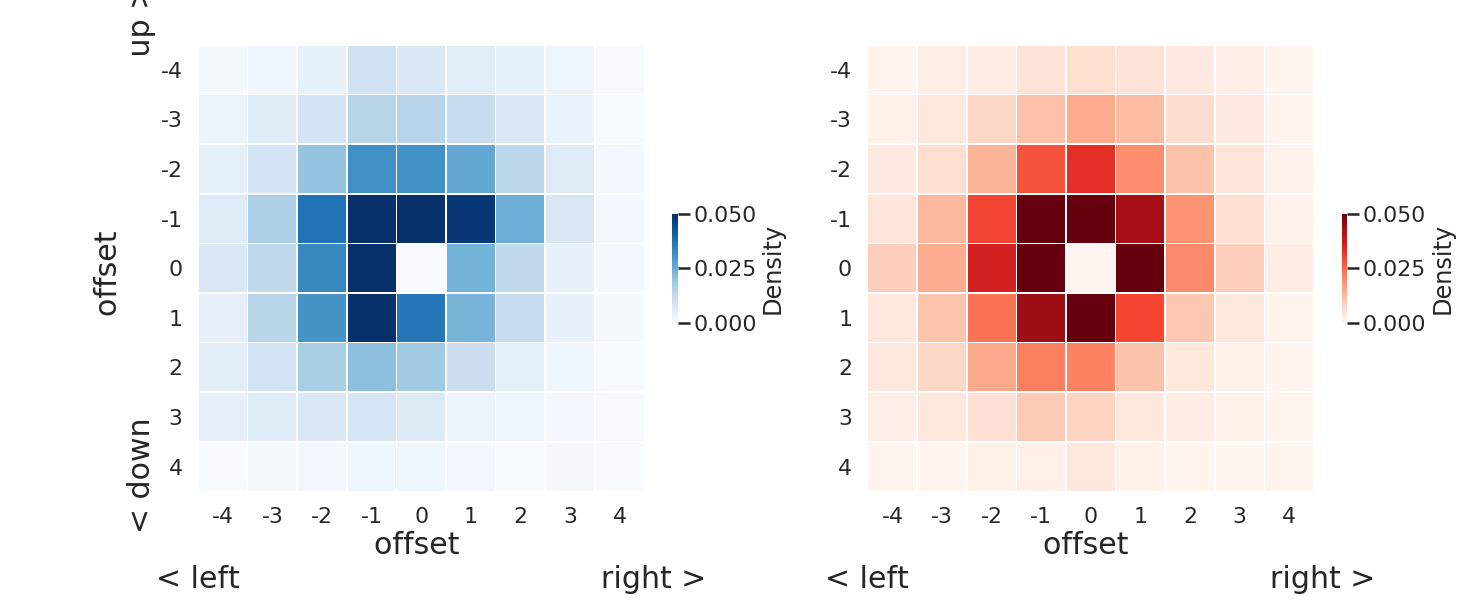
\includegraphics[scale=0.25]{source/figures/results/shelf_grasp_offsets.png}
    \caption[]{Object displacement behavior for the two task types. The left panel (blue heatmap) shows the movement offset for the EASY trials, right panel (red heatmap) for HARD trials. The movement offset is defined as the difference of the row-wise and column-wise difference of the drop-off location and pickup location at the end and beginning of the action execution respectively. Negative numbers in the ordinate refer to the object movement being upward and negative numbers in the abscissa refer to object displacement being leftward. For the EASY trials, most objects are moved one row upward and one column leftward. For the HARD trials, the object movement is also upward and leftward. For both trials, a majority of the final location is in the immediate vicinity of the initial location of the object.}
    \label{figure:offset}
\end{figure}


\begin{figure}[h]
    \centering
    \subfloat[]{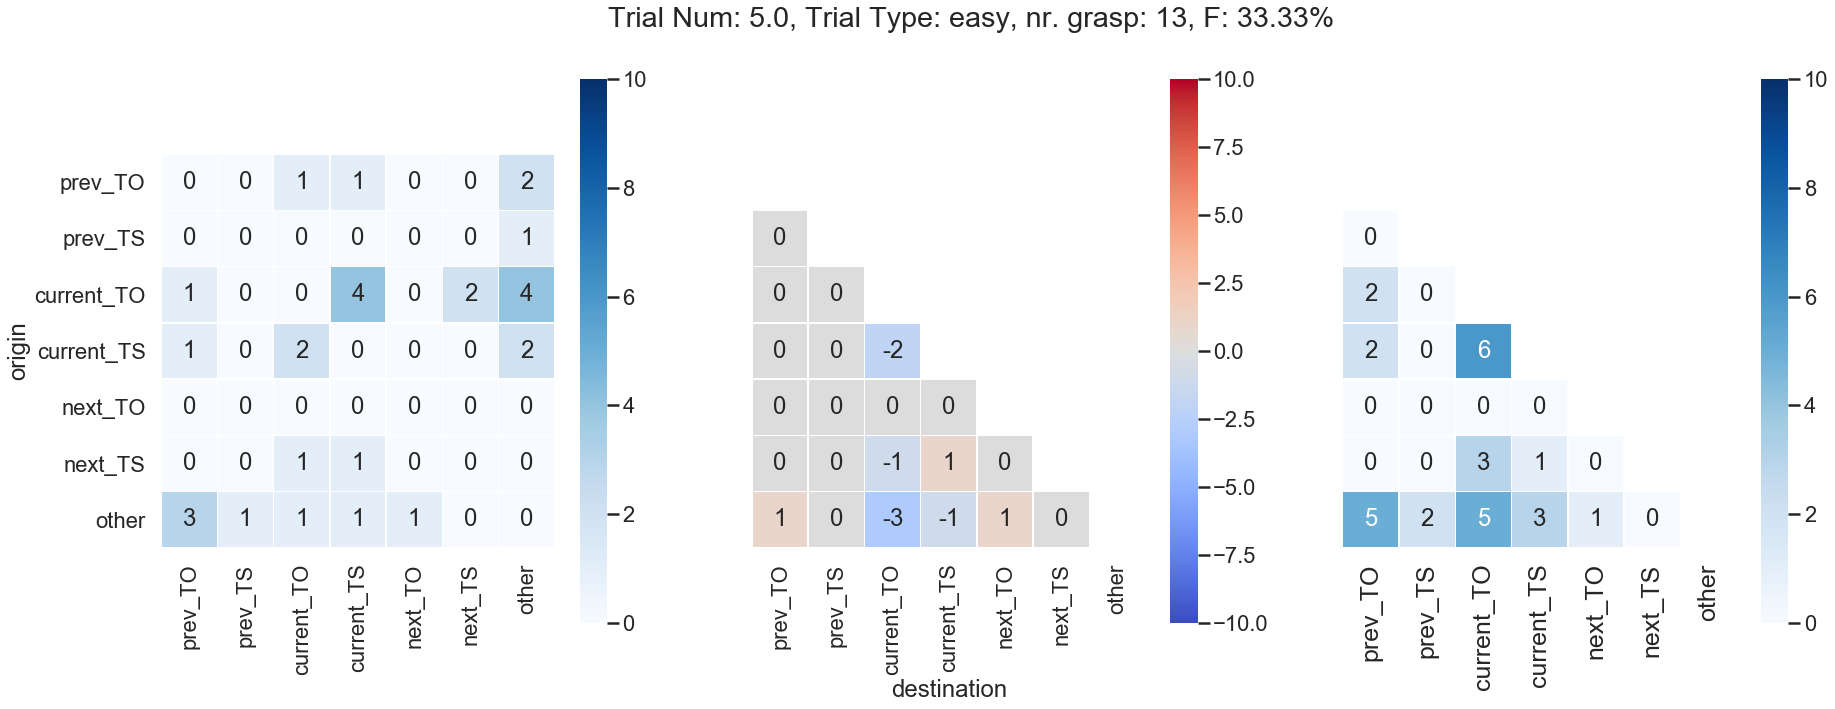
\includegraphics[width=0.7\linewidth]{source/figures/results/transition_matrix_trial_5_exe.png}
    \label{figure:transition_1}} \\
    \subfloat[]{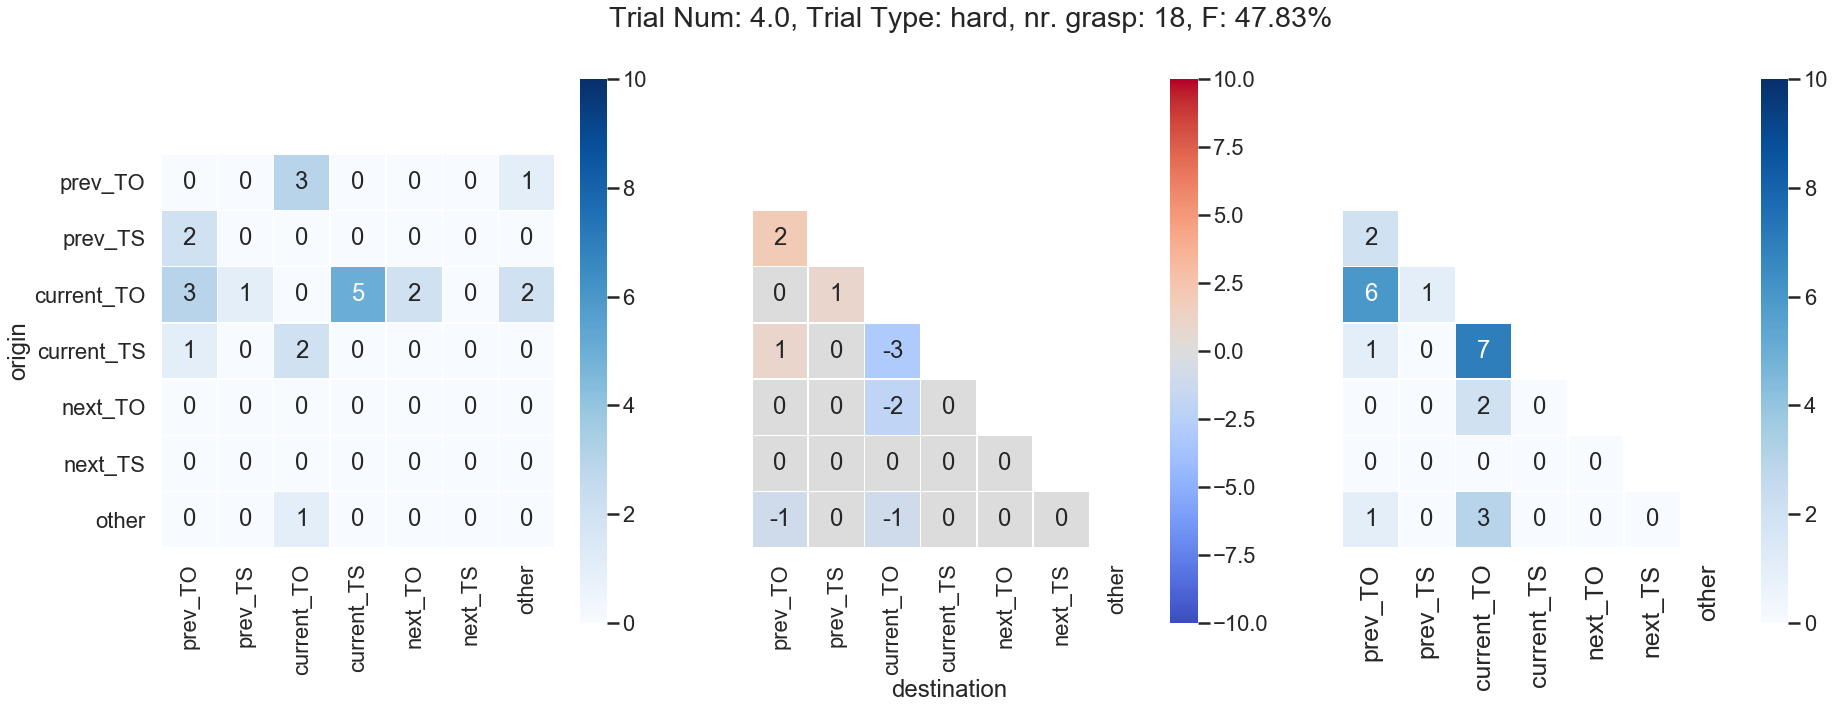
\includegraphics[width=0.7\linewidth]{source/figures/results/transition_matrix_trial_4_exe.png}
    \label{figure:transition_2}}
    \caption[]{Exemplar transition matrices for gaze switching between end of previous grasp and start of current grasp for the two trial types. The ordinate denotes the origin of the gaze i.e. where the gaze was before and the abscissa denotes the destination of the gaze. The diagonal contains zero as the transition is defined as a saccade from one ROI to another and not re-fixations on the same ROI. The left panel shows the transition matrix, A. The middle panel, shows the net transitions (A\textsubscript{NET}) The positive number in the matrix denotes transitions from source ROI to destination ROI, whereas the negative numbers reverse the direction of transition. The right panel shows the total transitions (A\textsubscript{TOTAL})  made between the 7 regions of interest. The F-value in the in the figure title refers to the relative number of net transitions compared to total transition matrix along with the the number of grasps and the trial type.  \\
    Panel \protect\subref{figure:transition_1} shows the transition matrix for gaze switching in an EASY trial with 13 grasps/object displacements. As shown in the middle panel, in the trial, there is 1 net transition are made to prev\_TO to other, whereas 3 transitions are made from current\_TO to 'other'. The right panel shows the total number of transitions made between the the ROIs. This tells us the that a majority of the transitions are from 'other' sources to the regions of interest. The F value for this trial shows that 33.33\%  net transitions are present in the total transitions.\\
    Panel \protect\subref{figure:transition_2} shows the transition matrix for gaze switching of in a HARD trial with 18 grasps/object displacements. As shown in the middle panel, in the trial, 8 transitions are made from prev\_TO to other, and 8 transitions are made from 'other' to current\_TO. And other ROI have close to net zero transitions. The right panel shows the total number of transitions made between the the ROIs. It tells us the that a majority of the transitions are from current\_TO to the current\_TS. The F-value for this trial shows that 47.83\%  net transitions are present in the total transitions.}
    \label{figure:transition_matrices_exe}
\end{figure}

\begin{figure}[h]
    \centering
    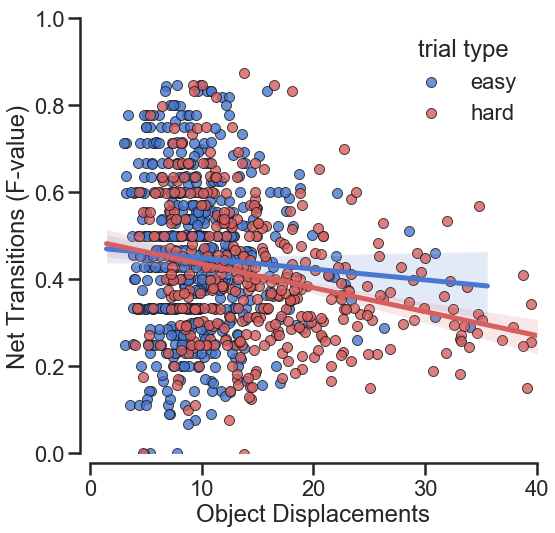
\includegraphics[width=0.3\linewidth]{source/figures/results/gaze_guidance_v_grasps_execution.png}
    \caption[]{Gaze guidance behavior vs. number of object displacements. Figure shows a scatter plot of the relative net transition (F-value) vs. number of object displacements per trial and subject differentiated the two trial types EASY(blue), HARD(red). Each point refers to one trial and it's F value vs. the number of object displacements in that trial. The lines denote the regression fit and the shaded region denotes 95\% confidence interval. F-values for both trial types decrease with increasing number of object displacements. Specifically, higher number of object displacements in a trial is correlated with lower gaze guidance. Pearson correlation $\rho$= -0.05 (p = 0.16) for EASY trials and $\rho$ = -0.25 (p<0.000) for HARD trials.}
    \label{figure:F_value_exe}
\end{figure}

\begin{figure}[]
    \centering
    \subfloat[]{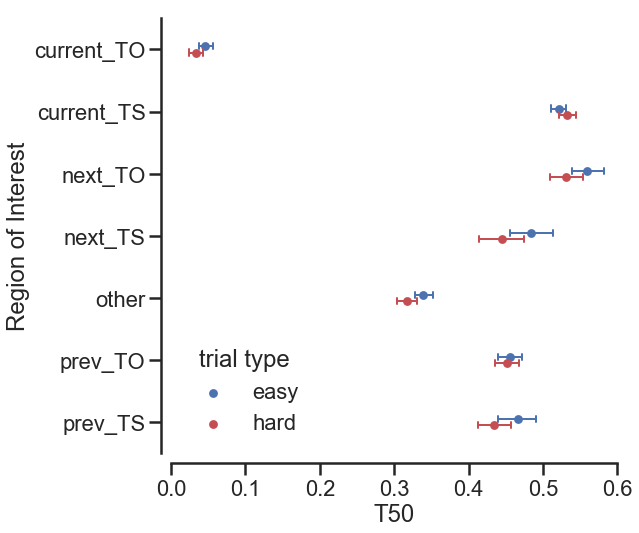
\includegraphics[width=0.3\linewidth]{source/figures/results/t50_subject_execution.png}\label{figure:t50_sub_exe}}
    \subfloat[]{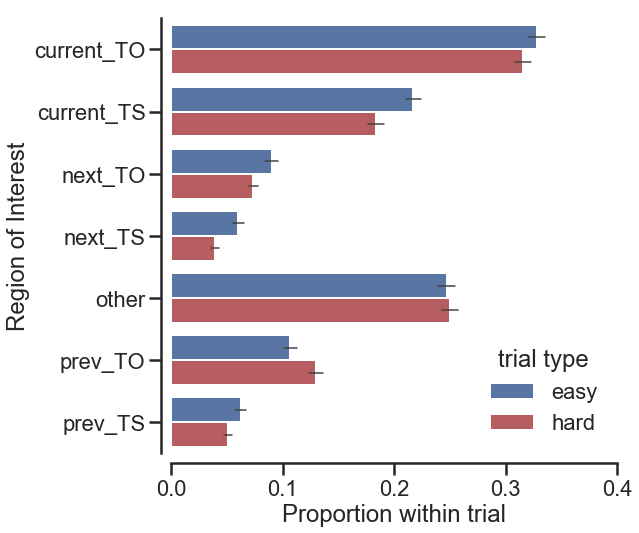
\includegraphics[width=0.3\linewidth]{source/figures/results/first_fix_roi_execution.png}\label{figure:t50_exe_fix_prop}}
    \caption[]{ T50 for the action execution epochs. In order to capture the latency T50 as an estimator for latency of first fixation on the 7 ROIs per trial. 
    Panel \protect\subref{figure:t50_sub_exe} shows the mean and 95\% confidence interval of T50 estimate for each trial. Blue points show the mean T50 for EASY trials and red points show the the T50 for the HARD trials.
    Panel \protect\subref{figure:t50_exe_fix_prop} shows the proportion of first fixations on each of the 7 ROIs. Blue bars show proportion of first fixation on given ROI for EASY trials, red bars for HARD trials. Error bars indicate 95\% confidence interval.
    }
    \label{figure:t50_subject_exe}
\end{figure}

\begin{figure}[h]
    \centering
    \subfloat[]{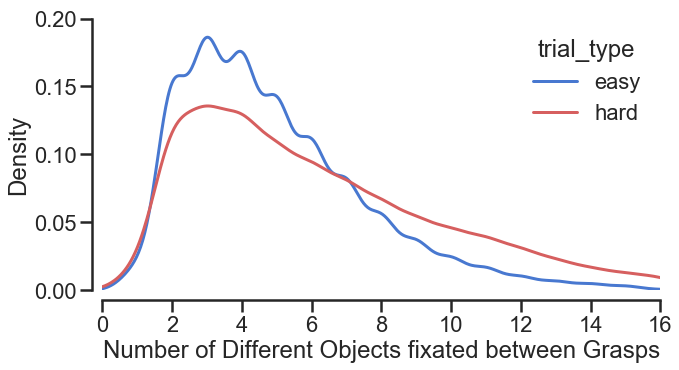
\includegraphics[width=0.5\linewidth]{source/figures/results/fixations_between_grasps.png}
    \label{figure:fix_bw_grasp}} 
    \subfloat[]{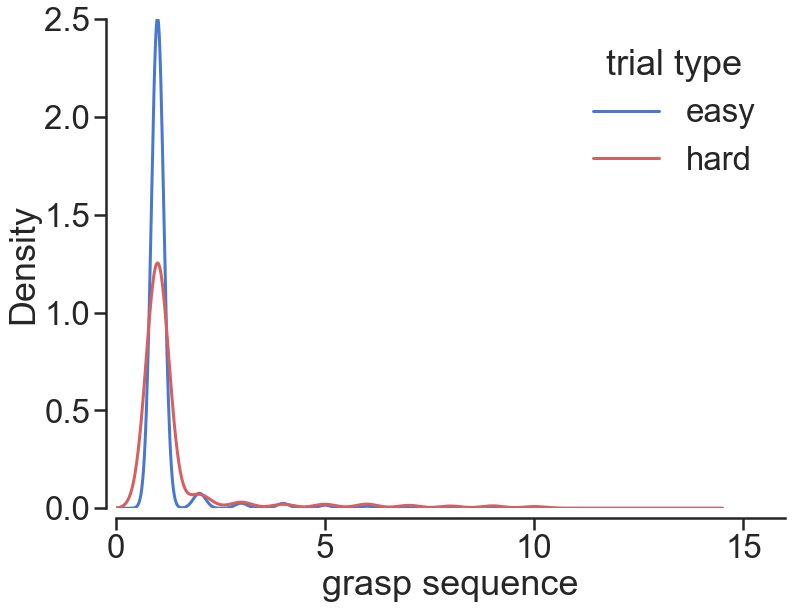
\includegraphics[width=0.4\linewidth]{source/figures/results/lookahead_distance_most_fixated.png}
    \label{figure:most_fixated}}\\
    \subfloat[]{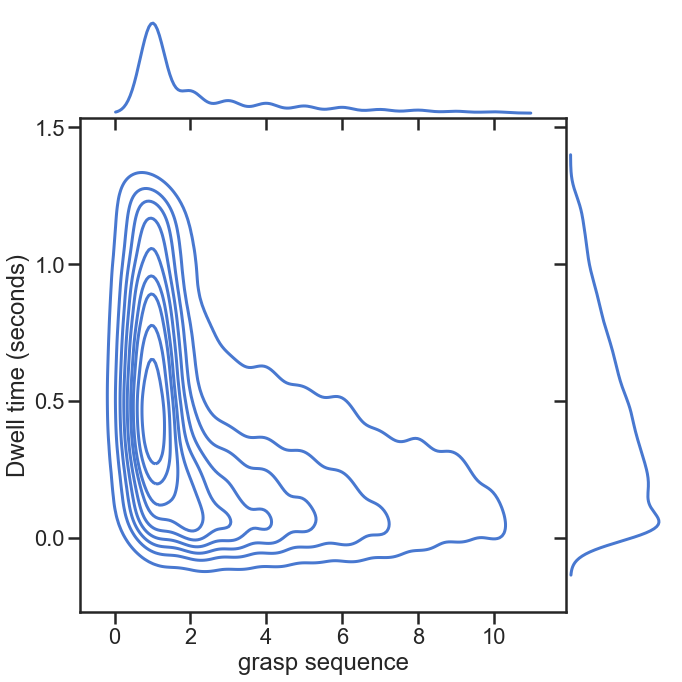
\includegraphics[width=0.4\linewidth]{source/figures/results/lookahead_distance_duration_easy.png}
    \label{figure:tla_easy}}
    \subfloat[]{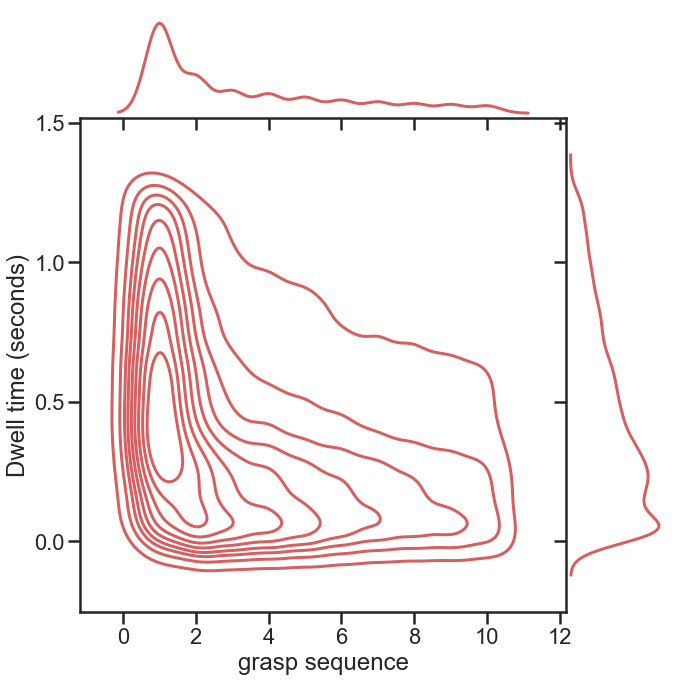
\includegraphics[width=0.4\linewidth]{source/figures/results/lookahead_distance_duration_hard.png}
    \label{figure:tla_hard}}
    \caption[]{\protect\subref{figure:fix_bw_grasp} shows the probability density of unique objects fixated on between consecutive grasps for the two trial types EASY (blue) and HARD (red). For both EASY and HARD trials, maximum probability density of fixation is on three unique objects in the scene. \protect\subref{figure:most_fixated} shows the probability density of the most fixated object in a grasp sequence. For both EASY and HARD trials, the maximum probability of density is on the object that is immediately grasped next, this shows that between two grasp onsets, maximum attention is allotted to the object that is next in line to be grasped. 
    \protect\subref{figure:tla_easy}\protect\subref{figure:tla_hard} show the joint probability density of the dwelling time (total fixation duration) on an object between consecutive grasps and it's position in the relative grasp sequence for EASY and HARD trials respectively. The figure also shows the marginal probability density of the dwelling time  on an object and it's relative position in grasp sequence. The abscissa refers to the relative grasp sequence of a fixated object i.e., when the grasp sequence of a fixated object is 1 the object is grasped next or when the grasp sequence is 2 the fixated object is grasped one after the next grasp.  the The figure shows that the dwelling time is highest on the object that is immediately next in line to be grasped. The dwelling time reduces linearly on the objects that are upcoming in the relative grasp sequence. The differences in the EASY and HARD trials can be explained by the higher number of objects fixated on between grasps in the HARD trials as shown in \protect\subref{figure:fix_bw_grasp}
    }
    \label{figure:planning_behavior}
\end{figure}


\begin{figure}[h]
    \centering
    \subfloat[]{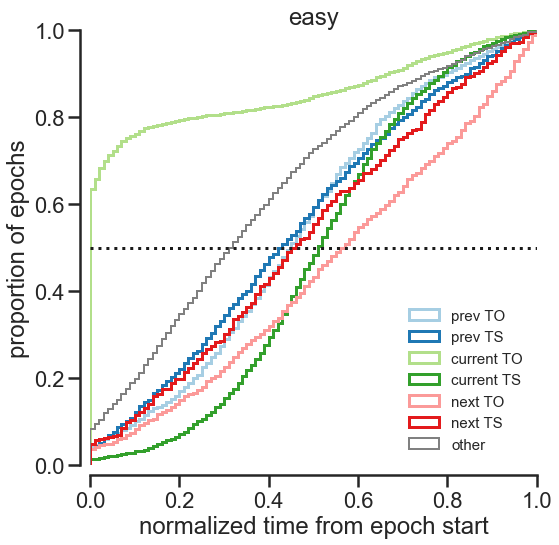
\includegraphics[width=0.3\linewidth]{source/figures/results/t50_easy_execution.png}
    \label{figure:t50_easy_exe}}
    \subfloat[]{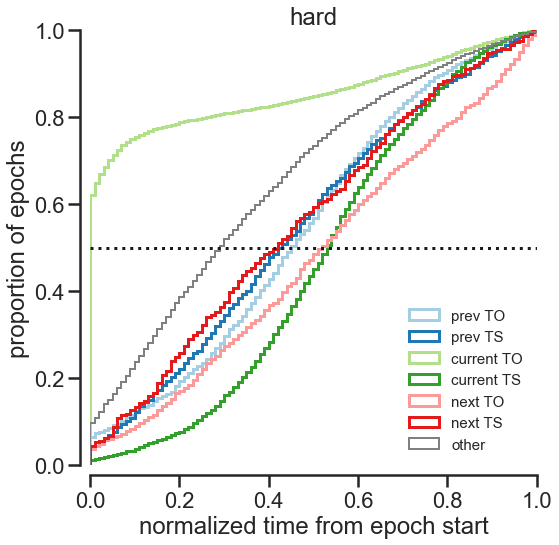
\includegraphics[width=0.3\linewidth]{source/figures/results/t50_hard_execution.png}
    \label{figure:t50_hard_exe}} \\
    \caption[]{Cumulative distributions of time of first fixation on the 7 regions of interest for the action execution epochs. The dotted line indicates time required in 50\% of all epochs to first fixation on the ROIs. The time taken for first fixation on each ROI can be  used to determine the attention attraction power of a region of interest i.e. the time taken to saccade to the region of interest.\\
    Panel \protect\subref{figure:t50_easy_exe} shows the cumulative plots for the 7 ROIs for the EASY trials. In 50\% of the action execution epochs the 7 ROIs are fixated on within half time of the epoch duration. At the 50\% mark, the curves indicate the latency of gaze shift from the current\_TO, other objects and shelves, closely followed by the previous target object and shelf (prev\_TO, prev\_TS), then to next target shelf (next\_TO), current target shelf (current\_TS) and next target object (next\_TO). This is indicative of attention equally distributed on the 6 ROIs and no selective preference for any one object or shelf in the task sequence during the later stages of action execution epoch.\\
    Panel \protect\subref{figure:t50_hard_exe} shows the cumulative distribution of the time to first fixation on the 7 ROIs for HARD trials. In 50\% of the action execution epochs, a similar trend is seen as in the EASY trials.
    }
     \label{figure:t50_overall_exe}
\end{figure}



\begin{figure}[h]
    \centering
    \subfloat[]{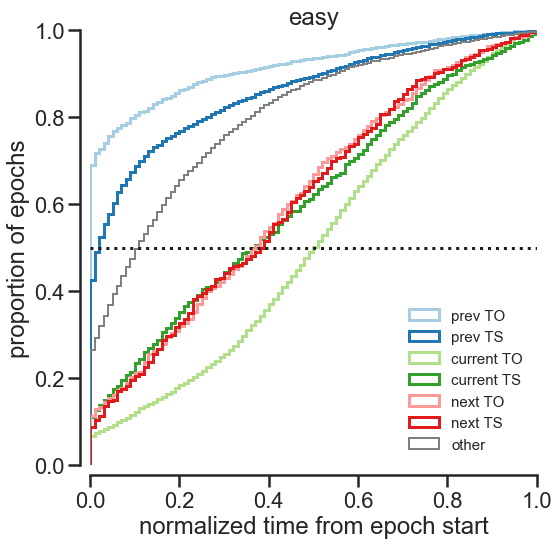
\includegraphics[width=0.25\linewidth]{source/figures/results/t50_easy_planning.png}
    \label{figure:t50_easy_plan}}
    \subfloat[]{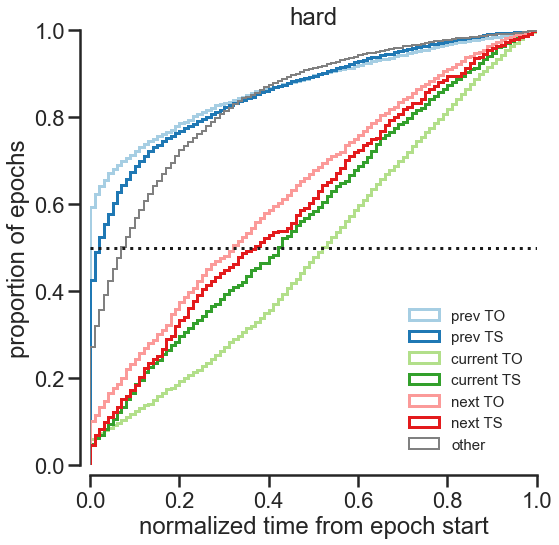
\includegraphics[width=0.25\linewidth]{source/figures/results/t50_hard_planning.png}\label{figure:t50_hard_plan}}
    \caption[]{Cumulative distributions of time of first fixation on the 7 regions of interest for action planning epoch. The dotted line indicates time required in 50\% of epochs to first fixate the ROIs.
    Panel \protect\subref{figure:t50_easy_plan} shows the cumulative plots for the 7 ROIs for the EASY trials. In 50\% of the epochs gaze is directed early to the previous target object and shelf. Further, gaze moves to other objects/shelves in the scene which is then followed by close fixations on next target object and shelf and lastly to the current target object well before the action on the object is executed. This is indicative of attention sequentially moving from one ROI to the next.
    Panel \protect\subref{figure:t50_hard_plan} shows the cumulative distribution of the time to first fixation on the 7 ROIs for HARD trials. In 50\% of the grasp epochs, The latency of first fixations on the ROIs remains roughly similar to the action planning epochs of the EASY trials, where the early fixations are on the previous target object and shelf and the last on the current target object before being manipulated.}
     \label{figure:t50_overall_plan}
\end{figure}
\end{document}
% \endinput

